\documentclass[12pt,a4paper,oneside]{report}
\usepackage{suthesis-2e}
\usepackage[a4paper]{geometry}
\usepackage{amssymb,amsmath,amsthm}
\usepackage{graphicx}
\usepackage{url}
\usepackage{hyperref}
\usepackage{tikz}
\usetikzlibrary{shapes,arrows}
\usepackage[utf8]{inputenc}
\usepackage{float}
\usepackage{longtable}
\usepackage[style=numeric,sorting=none,useprefix,hyperref,backend=bibtex]{biblatex}

\graphicspath{{imgs/}}
\addbibresource{mybib.bib}



%definzioni tikz
\tikzstyle{block} = [draw,fill=black!5, rectangle, minimum height=1.5em, minimum width=4em]
\tikzstyle{invis} = [draw=none]
\tikzstyle{dot} = [draw,fill=black, circle]
\tikzstyle{ball} = [draw,fill=black!5, circle]

\begin{document}
\title{
Artificial Intelligence based \protect\\
Narration Engine \protect\\ 
to improve engagement \protect\\ 
\vspace{8pt}
and to support long term exergaming}
\author{Riccardo Cantoni}
\dept{Corso di Laurea in Informatica} 
\anno{2017-2018}
\matricola{901564}
\relatore{Prof. Alberto Borghese}
\correlatore{Dr. Jacopo Essenziale, Dr. Renato Mainetti}
\copyrightyear{2018}
\beforepreface
\prefacesection{Preface}
This thesis tells you all you need to know about...
\prefacesection{Acknowledgments}
I would like to thank...
\afterpreface

\pagebreak

\chapter{Introduction}
\section{Goals and Applications}

Today, Narrative is produced and consumed through a variety of mediums, ranging from spoken words to videogames, from paper books to virtual reality. While it is usually considered to be a form of entertainment, it is, and has always been, employed to achieve other goals.

A long standing example is the field of Education: for centuries folktales have been used as a means to convey teachings from one generation to another \cite{moraltales}. More recently systematic studies of pedagogy allowed for more complex ways of employing Narrative in teaching \cite{pedagogy}.
The benefits given by the employment of Narrative in Education are multiple: stories can inherently increase appeal and engagement, while showing a certain cultural transcendence \cite{narrationlearning}. 

Also, even more recently, the concept of Serious Games draws a new connection between the narrative-rich world of video games and the field of education.

The field of Medicine is an other example of the use of narrative in other contexts: as a means to facilitate all the inherently necessary human interactions \cite{narrativemedicine}, as well as for more technical applications in psychological therapy \cite{psychotherapy}.

\bigskip

This work focuses on the task of generating Narrative \textit{procedurally}, via an algorithm. This would have numerous advantages, while also introducing new challenges.

\bigskip

\textit{Procedural Content Generation} is the \textit{algorithmic creation of content with
limited or indirect user input} \cite{pcg}. It is a concept often applied and originating from the field of games, but with implications spanning any other area in which content can be generated automatically.

The main advantages of generating contents procedurally include an increased efficiency of the content generation process (not requiring humans, or requiring less human work), an increased volume of content, as well as an increase in variety in the produced contents \cite{pcg}.

\bigskip

A context that would benefit strongly from a system capable of generating stories procedurally is one in which a large volume of material needs to be generated, while ensuring the adherence of every story produced to certain constraints.  In cases like this, a single human author would not be capable of maintaining the production rates required, while a large group of human writers would be difficult to coordinate so that the output is always acceptable.

An automated procedure, however, would be able to produce material at a much faster rate, while guaranteeing output validity if designed correctly. Also it could be constructed in such a way that allows for the tailoring of each story in response to a set of specified parameters.

The quality of the material produced poses a difficult challenge: how does one capture the essence of a "beautiful" story in a way that allows its formalisation into a piece of code? this is an open problem which sees many attempted solutions, but no final answer (see section 1.2).

\bigskip

From the analysis of literature done within this work, two projects emerged, that offer the possibility of employing procedurally generated narrative in a very useful manner: enhancing and enriching systems aimed at improving the health, autonomy and quality of life of elderly people and other groups of patients.

In the next sections these two project will be briefly presented, in order to explain how procedural narrative can be integrated in their architecture and how it could be useful.

\subsection{MoveCare Project}
\textit{MoveCare} \cite{movecare} is a three-year EU-backed project, aiming to help elderly people to remain autonomous and continue living in their own homes, instead of needing to move to a nursery home.

The project is aimed at elderly people who are classifiable as Pre-Frail. Frailty is an ageing-related syndrome, common in geriatric patients, accompanied by a high risk of a disastrous decline in the overall health of a person \cite{frailty}. Pre-frail people are vulnerable to becoming frail, if their cognitive and physical decline, boosted by ageing, continues.

The project tries to prevent or offset the transition from pre-frail to frail in elderly people, by promoting different kinds of activities in their day-to-day life and monitoring their status.

``MoveCare integrates an existing robotic platform with a domotic system, smart objects, a virtual community and an activity center, to provide, through artificial intelligence, assistance, activities and transparent monitoring to the elder at home. MoveCare can be tailored to each elder thanks to a modular design. It is completely unobtrusive as MoveCare does not require the elder to wear any particular device."

In the context of the project a hierarchical platform is being developed and tested, which integrates an array of different elements and functionalities:

\begin{itemize}\setlength{\itemsep}{8pt}
\item \textit{Activity Center}: the component offers the elder a variety of activities, and supports him or her in their performing, designed to exercise physical, cognitive and social skills.\\
Motivation, engagement and longevity of the experience are to be reinforced through the means of a gamification system and automatic narration techniques.
\item \textit{Virtual Community}: the elders are put in contact with each other and with caregivers, through this community system, in order to promote socialisation and avoid isolation, which is a major factor in the degradation of cognitive abilities.
\item \textit{Virtual Caregiver}: this component aids clinicians and caregivers in assisting the elder, while supporting and automating some features of the assistance activity. It collects and processes data using machine learning and artificial intelligence techniques, suggests activities through the Activity Center, while adjusting them to better suit the physiological and cognitive status of the elder, provides assistance in finding lost objects and in following a diet or a therapy.\\
The Virtual Caregiver also provides caregivers and clinicians with data pertaining the status of the elder.
\item Assistive Robot: the Giraff \cite{giraff} robot is employed as an active companion to the elder, capable of autonomous navigation. It is used to provide companionship and feedback, while also being a valuable tool to render assistance in cases of need.
\item Sensorised Objects: common items of everyday's life, ranging from pens and glasses to walking sticks are sensorised to gather data about the activities of the elder, while monitoring more clinical parameters such as gait stability and handling pressure. These data are combined together and are used by clinicians, caregivers and other MoveCare components, to monitor variations in the health status of elder, as well as to suggest specific beneficial activities.
\item Domotics: domotic sensors, voice analysis and other data gathering systems provide measurements useful for the early detection of physical and cognitive decline. 
\end{itemize}

\begin{figure}[H]
\begin{center}
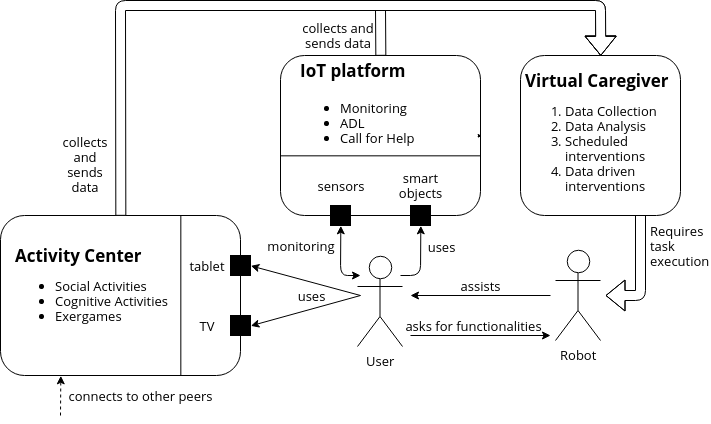
\includegraphics[width=13cm]{giraffmovecare}
\caption{Architecture of MoveCare \cite{movecareimage}}
 \label{fig:movecare}
 \end{center}
\end{figure}

\pagebreak

\subsection{REWIRE Project}
REWIRE \cite{rewire} is a EU-financed project. It ``develops, integrates and field tests an innovative virtual reality based rehabilitation platform system based on a multi-level rehabilitation platform.".

Its aim is to provide patients that have already been discharged from hospitals with a means to continue the needed rehabilitation programme at home, with minimal effort and at minimal costs. Its architecture encompasses three main components:

\begin{itemize}\setlength{\itemsep}{8pt}
\item \textit{Hospital Station}: is used at hospitals by clinicians. It allows them to define, schedule and tune the rehabilitation programme to be followed by each patient. It also receives and aggregates data produced by the patient so that clinicians can monitor his or her status and better refine the specific therapy.
\item \textit{Patient Station}: is the means through which a patient can follow a rehabilitation programme, by playing a series of \textit{Exergames} on a TV set. Patients are automatically guided by the system through these activities in order to prevent risks and maladaptation. Data pertaining to the motion of a patient are gathered during the activities.
\item \textit{Networking Station}: allows for collection, storing and analysis of data, making them available to clinicians and researchers for study.
\end{itemize}

Exergames are videogames that require physical exercise. They have been marketed for entertainment since the 1980's but have enjoyed a wider diffusion only in the last decade, due to major advancements in motion tracking technology \cite{tanaka}. Other than in the field of entertainment, exergames have been employed successfully in the field of Medicine, especially as tools for data gathering and the measurement of health parameters \cite{exergmeasure}, for rehabilitation \cite{exergrehab} \cite{pirovano17} and for therapy \cite{exergtherapy}.

\begin{figure}[H]
\begin{center}
\caption{An Exergame for the rehabilitation of the legs}
 \label{fig:exergame}
\includegraphics[width=13cm]{pumpthewheel}
\end{center}
\end{figure}

In the case of REWIRE, the patient carries out a therapeutic task in the game world through his or her avatar. Motion is recorded through devices such as Microsoft's \textit{Kinect} and the balance board \textit{TYMO} by Tyromotion, and is translated into movements of the avatar. 

These games are the means through which patients carry out their rehabilitation activity. Each game is designed to respond to a specific therapeutic need, such as exercising specific muscles in a specific way, with a focus on whether the movement is carried out precisely in the correct way \cite{pirovano17}.

They are meant to make a repetitive, therapeutic task less abstract, by building an entertaining interface around it. 

\pagebreak

\subsection{Gamification For Long-term Engagement}
The matter of long-term motivation and engagement is crucial to projects of this kind: users, or patients, should keep interacting with these systems for prolonged periods of time. In the case of REWIRE, patients might have to follow a long rehabilitation period of several months, while as for MoveCare, elders should conceivably make use of the system for the entirety of their third age.

Since the effectiveness of these systems depends on the user's continuous participation in the activities, it is necessary to develop solutions to reinforce its interest in them. This lasting motivation becomes therefore a factor of major importance in the lasting effectiveness of the service offered.

\bigskip

The range and variety of activities available to these users is forcibly limited. Especially in the context of physical rehabilitation, each user is presumed to repeat the same limited set of exercises several times.

The task of maintaining long-term engagement is particularly challenging under these conditions, because of the inherently repetitive nature of some activities, together with the desired time span of their usage.

%TODO intrinsic extrinsic start
The ways in which motivation is increased have been subject of extensive studies in the field of social psychology. A distinction is made between \textit{intrinsic}, or \textit{internal}, and \textit{extrinsic}, or \textit{external} motivation.

The difference lies in where the motivation comes from: in the case of intrinsic motivation, the drive comes from within the activity itself, and the interest or satisfaction that derive from it \cite{vallerand92}.

In the case of extrinsic motivation, instead, external elements promote a behaviour indirectly, by giving additional goals that require said behaviour to be reached. This way, one sees the activities a means to an other end, rather than a driving force in itself \cite{vallerand92}.

\bigskip

For instance, a student could be motivated in studying with commitment because of an interest in the subject or the sense of pleasure and reward coming from the activity itself (intrinsic motivation). Or, the motivation could come from the desire of avoiding punishment, or obtaining some other reward, or from a sense of duty (extrinsic motivation).

\bigskip

Studies show that both types of motivation can be effective in reinforcing a desirable behaviour. However, extrinsic motivation can in some cases be have a detrimental effect, as individuals perceive it as externally regulated or alien to the activity \cite{decharms68} \cite{ryan2000}.

This limit is not shared by intrinsic motivation \cite{ryan2000}.

\bigskip

An approach that has been used to address the issue of engagement is the implementation of Gamification techniques. Gamification is defined as ``using Game Design elements in non-gaming contexts" \cite{deterdinggamification}. 

Gamification works by introducing elements reinforcing extrinsic motivation, especially to activities that struggle in generating intrinsic motivation, perhaps because of their repetitiveness or their lack of appeal \cite{seaborn2015gamification}.

%TODO intrinsic extrinsic end

Studies have shown how gamification can be effective in reinforcing desirable behaviours and the volume of user activity \cite{hamari14} in many fields of application, including:

\begin{itemize}\setlength{\itemsep}{8pt}
\item Learning: gaming elements can be added to pre-existing learning environments, to improve their effectiveness. Similarities between the process of learning a complex subject and playing a game facilitate this application. Students learn how to solve complex problems, unveiling more and more information as the game progresses towards a clearly defined goal \cite{gamificationlearning}.

Also, elements that are typical of the field of gaming, such as the concept of \textit{Flow} (A mental state of complete immersion and concentration upon a specific task) have proven to be successful in enhancing the effectiveness of learning systems\cite{gamificationlearning}. Competition, progressive rewards, and tools for socialization have also been applied with positive results \cite{gamificationlearning2}.

\item Crowdsourcing: the practice of externalisation of parts of the processes of an enterprise is more and more common. Gamification methods are used to increase user engagement, support user activities and reinforce useful user behaviours \cite{gamificationcrowdsourcing}. Even monetary rewards have been introduced.

\item Physical exercise: gamification is employed to increase adherence and user commitment  \cite{gamificationexercise}.

\item User Engagement: studies show that implementing gamification techniques in various contexts increases the volume of user activity, even after a time span of years \cite{gamificationengagement1}.

Goals of this approach include increasing the volume of trade on e-commerce websites \cite{gamificationecommerce}, and engaging the employees of an enterprise while simultaneously reinforcing positive behaviours and increasing their productivity \cite{gamificationenterprise}.
\end{itemize}

Gamification is currently being designed to be integrated into MoveCare to respond to the specific issue of user engagement. The system is currently undergoing development. 

However, a generic structure has been already laid down.

\begin{figure}[H]
\caption{Gamification system in MoveCare}
 \label{fig:gamificationmovecare}
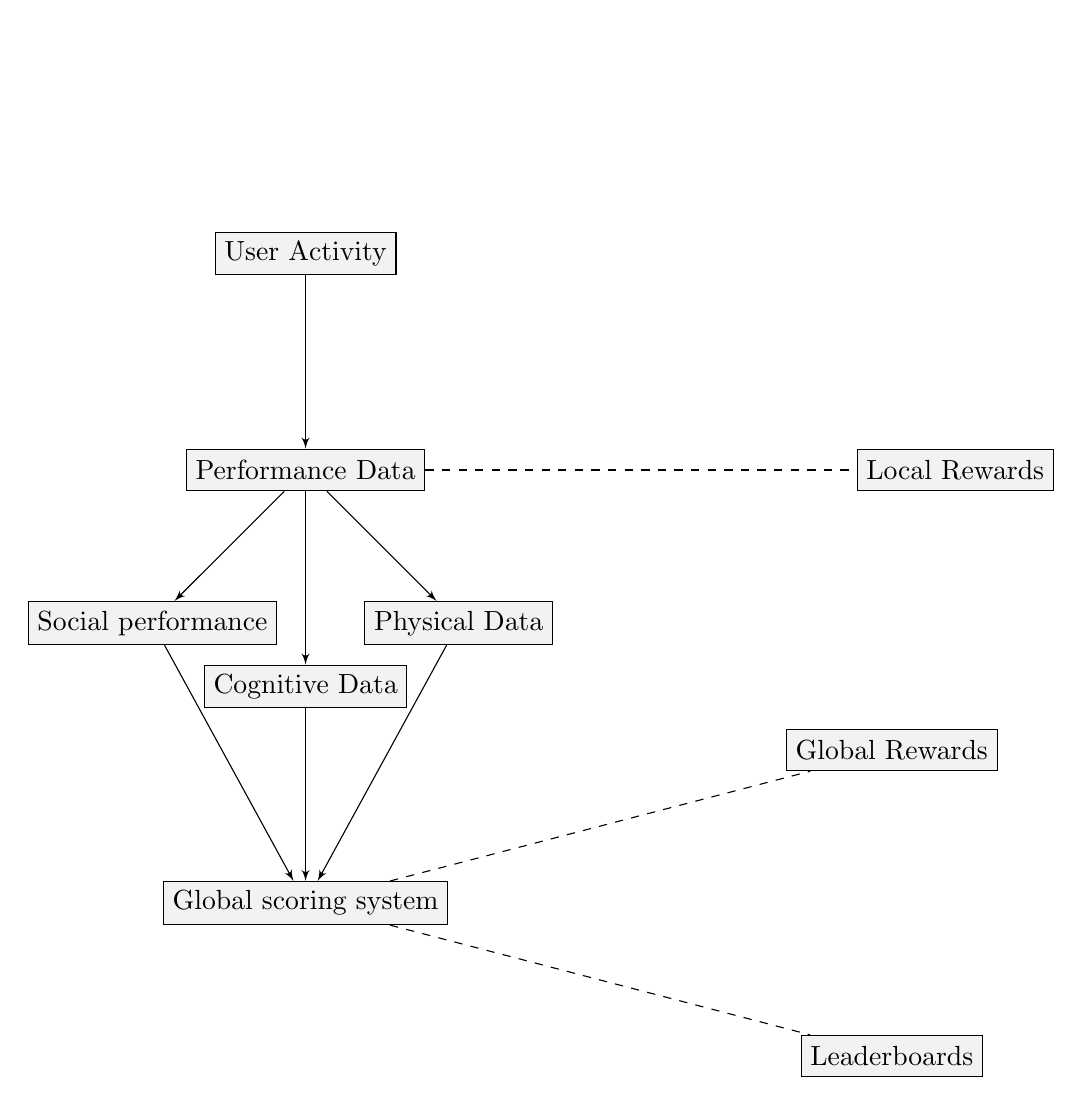
\begin{tikzpicture}[auto, node distance=2.75cm,>=latex']
 % nodes
    \node [invis, name=invis] {};
    \node [block, below of = invis, name = activity] {User Activity};
    \node [block, below of = activity, name=performance] {Performance Data};
    \node [invis, right of=performance, name=loc1]{};
    \node [invis, right of=loc1, name=loc2]{};
    \node [block, right of = loc2, name=local] {Local Rewards}; 
    \node [block, below left of = performance, name=social] {Social performance};
    \node [block, below of = performance, name=cognitive] {Cognitive Data};
    \node [block, below right of = performance, name=physical] {Physical Data};
    \node [block, below of = cognitive, name=global] {Global scoring system};
    \node [invis, right of=global, name=glob1]{};
    \node [invis, right of=glob1, name=glob2]{};
    \node [block, above right of = glob2, name=globalrw] {Global Rewards};
    \node [block, below right of = glob2, name=leaderboards] {Leaderboards};
    % edges
    \draw [->] (activity) -- node[] {} (performance);
    \draw [->] (performance) -- node[] {} (social);
    \draw [->] (performance) -- node[] {} (physical);
    \draw [->] (performance) -- node[] {} (cognitive);
    \draw [->] (social) -- node[] {} (global);
    \draw [->] (physical) -- node[] {} (global);
    \draw [->] (cognitive) -- node[] {} (global);
    \draw [dashed] (performance) -- node[] {} (local);
    \draw [dashed] (global) -- node[] {} (globalrw);
    \draw [dashed] (global) -- node[] {} (leaderboards);

\end{tikzpicture}
\end{figure}

Performance of MoveCare users in the various activities are collected and used in a local system of rewards. Within this system, users who perform well unlock new features at the application level. 

Performance data are then aggregated in three main areas: Social, Physical and Cognitive, following the three main focuses of MoveCare. This aggregated data is then further processed into a global scoring system.

Users who perform well at the global level access global rewards.
Also, a leaderboard system allows them to compare their performance and score with that of other users, fostering competition.

\pagebreak


\subsection{Automatic Narration}

While the employment of gamification can be effective in reinforcing engagement, other options are available.

In particular, gamification works by adding extrinsic motivation to an activity. This, as stated in the last section, is not always effective, and can be even detrimental in some cases.

\bigskip

Automatically generated narrative can be employed as a tool to strengthen and reinforce the engagement and commitment of users. Integrating activities in a narrative structure would be a means to increase intrinsic motivation \cite{green2004understanding}, by making the participation of a user more interesting and rewarding \cite{sweetser2005gameflow}.

\bigskip

The goal of this work is to produce the means to employ automatically generated narrative to reinforce the engagement and commitment of users, in the context of the aforementioned projects MoveCare and REWIRE.

\bigskip

This involves experimenting with Story Generation, in order to design a system capable of encasing different activities into a narrative superstructure.

The concept of an exergame, especially, shows great potential in becoming an element within a story. Exergames are, in essence, simple scenes in which the user is the main character who is requested to perform a certain simple task, through the medium of a digital avatar. A careful design of the setting of an exergame, coupled with the appropriate narrative superstructure, allows it to become a section in a sequence of scenes constituting a narrative.

The task becomes then to generate a coherent, and possibly interesting, story from which individual scenes or sequences can then be mapped on exergames.

\bigskip

On the subject of coherence, a coherent story is really just a story that adheres to a set of predefined rules. Whatever architecture one decides to use, it must be defined in a way that only produces valid stories: a story in which the Prince \textit{eats} the Princess is, under normal circumstances, not valid, while one in which the Prince \textit{marries} the Princess is acceptable.

Clearly, the more constrains are required to define the specifics of desired stories, the more rules will need to be in place. This will impact negatively on the possible variety of outputs, by taking away elements from the output space of all possible stories. The issue of ensuring sufficient variety needs careful consideration.

Clearly, a complete story is made of a variety of highly differentiated scenes. The degree of variety in the set of exergames scheduled for a user to perform is much more limited: in fact, the number of physical exercises designed for the rehabilitation of a certain patient, or the activities made available in a health care system, is forcibly reduced. Moreover, it is not possible to map every conceivable story scene into a game or activity.

Also, the developing of new games and activities is a costly endeavour which is outside the scope of this work. Any procedure for the generation of narrative will therefore have to face severe limitations in the amount of story elements that can be mapped into user interactions.

One obvious path would be to restrict the set of scenes that can be used to compose a story so that it coincides with the set of available activities. This is, however, highly impractical: there are only so many ways in which to organise a small set of sequences until the overall narrative degrades into meaningless repetition.

\bigskip

A more sensible approach is to accept that not every story element will be translated into an activity: some scenes and events can be in fact delivered to the user through other mediums, being initially written text, and later perhaps images or even animations.

The final story would therefore appear to the user as a sequence of scenes in which activities with him or her as the protagonist are interleaved with text, images and such.

\bigskip

Still, the problem of variety remains. Given that activities constitute fixed scenes that are always the same, whatever story is going to be generated shall be strictly constrained by the necessity of incorporating these rigid elements. A way to address this issue is to build exergames in such a way that allows for the replacement of assets in the game scene at runtime. This way, the same activity could be dressed in different ways to increase variety, without incurring in the higher costs of the development of a new one.

For example, the same activity of moving one's body to avoid obstacles that are in the path of the avatar, can once become a scene in which the avatar is moving on a horse through a forest, and once one in which it is crossing a body of water on a boat. The mechanics would remain, and the activity itself would have the same effect on the health of the user. While the comparatively simple operation of replacing the assets would allow for the scene to be recycled in various narrative contexts.

This would in turn increase the size of the output space. The generator, under the same circumstances, would not be forced to only generate stories in which the hero travels through a forest, but could also generate some in which he travels on the ocean, or through a city, or a desert, and so on. This would allow for more varied and interesting stories.

\pagebreak

\subsection{Requirements}
Java was chosen as programming language to be used in this work. This ensures that it remains reasonably compatible with the systems explained above, as well as being easy to deploy and maintain.

The objective is to outline an architecture capable of generating narrative. The resulting stories should adhere to a set of constrains, defined to ease their applicability as means to improve engagement. They should:

\begin{itemize}\setlength{\itemsep}{8pt}
\item \textbf{Be coherent}: Coherence is a requisite for acceptance. Valid stories "make sense". They exhibit consistency and reliability, while character behaviour and events are consistent with the setting, without extreme deviations.

\item \textbf{Contain struggle}: moments of struggle are central in the dramatic structure of any narrative. They are necessary to provide the audience with a focus for their interest. Moreover, moments of struggle, seen as problems a character needs to overcome, represent a prime opportunity for the introduction of user activities, in which the user himself takes part in the resolution of the problem.

\item \textbf{Focus on a single character}: The applications of this system are in single-user contexts. Generating stories that have a single character as protagonist, around whom the entire plot revolves, makes it easier to associate this single user to the main character, so that him or her becomes directly the acting subject of any activity.
\end{itemize}

Given the desired properties that apply to the output, there are necessities pertaining to the system itself. Features of the generation architecture include:

\begin{itemize}\setlength{\itemsep}{8pt}
\item \textbf{Expandability}: while the purpose of this work is to outline the architecture of a Narration Engine, the prototype will have to be designed in a way that allows for its further development into a more complete piece of software, following the Software Engineering principle of "Design-For-Change" \cite{designforchange}.

\item \textbf{Customisability and Modularity}: the software must be built in a modular way, that allows for quick redefining and replacement of some of its functional parts in order to alter its behaviour. Requirements about the output can be changed or simply be defined more finely. 

A monolithic architecture would prove extremely expensive to adapt to the evolution of requirements, as well as to tailor to the specific needs of any real-world application.

\item \textbf{Programmability}: the system must allow for the specification of parameters for the generation process. The most prominent of these parameters is the definition of items that have to be part of the output. Since some story elements will be associated to real-world activities that carry a therapeutic meaning, a way is needed to specify whether some story elements must be present in the final story.
\end{itemize}

\pagebreak

\section{Structure of the Thesis}
Here is outlined the structure of this work:

\bigskip

\begin{itemize}\setlength{\itemsep}{8pt}
\item In chapter 2, the state of the art is reviewed: how human and machine can cooperate in the production of narrative, how the different levels of automation are classified, what level of automation is going to be achieved with the approach proposed.

Also, two sources will be explain in greater depth, being the theoretical bases on which the algorithmic structure proposed in this work is built upon.

\item Chapter 3 describes a first attempt at a narrative generation structure. The approach is explained, as well as the problems and obstacle that arose and eventually caused the abandonment of it.

\item The general architecture of the generation system is described in chapter four. What modules have been implemented, a recount of their function and how they interact with each other.

\item Chapters 5 and 6 describe how the system works, and offer some insight into how it was implemented. The first focuses on how the plot is generated, while the second on how said plot is transformed into readable text.

\item Chapter 7 is the conclusion: how the proposed approach is different from those present in literature, what are its strengths and limits. Also the last steps necessary in order to produce a deployable prototype are outlines, as well as suggestions on future works of refinement and improvement.
\end{itemize}

\chapter{State Of The Art}
\section{The Mixed Initiative Approach}

Computers are often used as a means to design, produce, share, visualize and consume narratives of various description. The degree of involvement of the machine in the life cycle of a narrative product can vary substantially.

There is a contribution, albeit minimal, even when a text editor is used to write a physical book. At the other end of the spectrum some forms of narrative entertainment, such as videogames, animation or films, require a more direct participation of the machine, starting from the generation process all the way to the moment of its consumption by the public.

\bigskip

The subject of this work has to do with the generation part of the process.

\bigskip

A computer cannot be the sole author of a creative work, but rather it needs the human factor to produce meaningful narrative \cite{lubart05}. Any procedural generation algorithm aiming to produce narrative needs inputs that can only come from humans and their endeavours. This necessary cooperation and interdependence between human and machine in a creative process is usually referred to as the \textit{Mixed Initiative} approach \cite{negroponte75}, in which both agents participate varyingly.

Before discussing the different degrees of automation that can be applied to the components of Narrative, it is necessary to define them precisely. A formal definition of the structure of a narrative work is given by Kybartas and Bidarra \cite{kybartasbidarra17}:

\begin{itemize}\setlength{\itemsep}{8pt}
\item \textit{Narrative} is defined by \textit{Story} and \textit{Discourse} \cite{abbott08}.
\item \textit{Story} is the content of the narrative: the events that constitute it, the \textit{Plot} and the setting in which they happen, the \textit{Space}.
\item \textit{Plot} is the collection of all the events that take place in the story \cite{kukkonen14}. These are organised in a temporal ordering, and are linked by causal relations.
\item \textit{Space} includes the physical setting, the characters, objects, props, and anything present in or affected by the events described by the \textit{Plot} \cite{ryan14}. Characters, objects and locations in which the story unfolds are usually grouped under the term \textit{Existents} \cite{chatman80}.
\item \textit{Discourse} is the specific way in which the story is recounted: the style of the narration, the ordering of the events, the pace, the linguistic choices.
\end{itemize}

\begin{figure}[H]
\caption{Structure of Narrative Components}
 \label{fig:narrativecomponents}
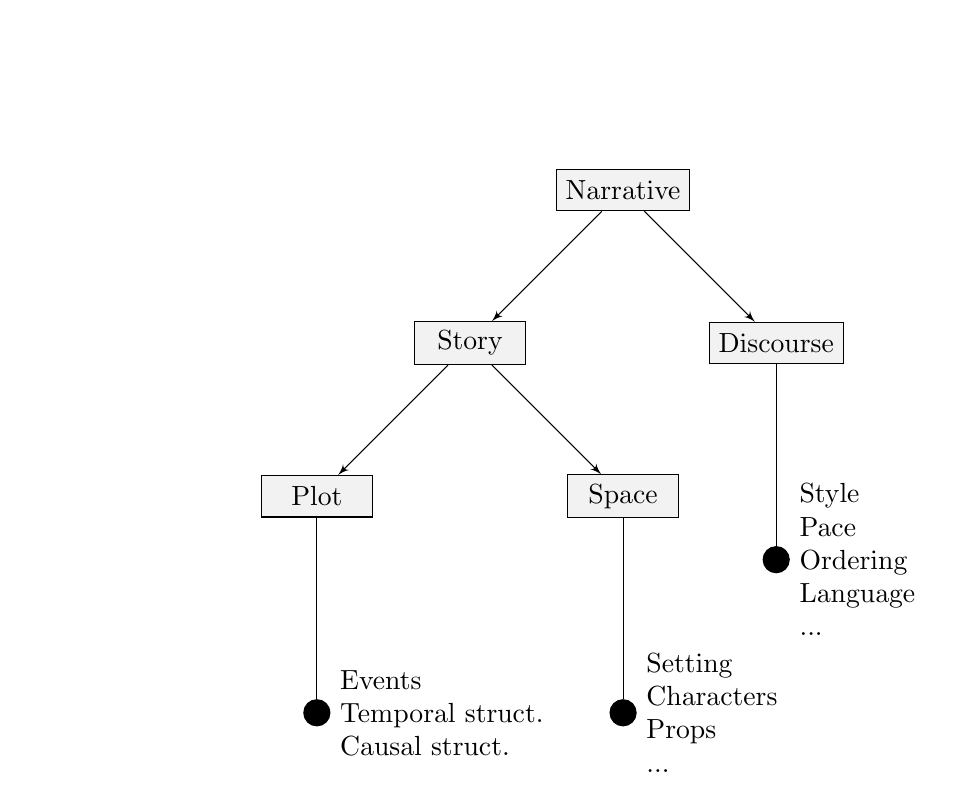
\begin{tikzpicture}[auto, node distance=2.75cm,>=latex']
 % nodes
    \node [invis, name=invis1] {};
    \node [invis, right of=invis1, name=invis2] {};
    \node [invis, right of=invis2, name=invis3] {};
    \node [block, below right of = invis3, name=narrative] {Narrative};
    \node [block, below right of = narrative, name =discourse] {Discourse};
    \node [dot, below of = discourse, label={[align=left]right:Style\\Pace\\Ordering\\Language\\...}, name = discourse2] {};
    \node [block, below left of = narrative, name =story] {Story};
    \node [block, below left of = story, name =plot] {Plot};
    \node [dot, below of = plot, label={[align=left]right:Events\\Temporal struct.\\Causal struct.}, name = plot2] {};
    \node [block, below right of = story, name =space] {Space};
    \node [dot, below of = space, label={[align=left]right:Setting\\Characters\\Props\\...}, name = space2] {};
    % edges
    \draw [->] (narrative) -- node[] {} (story);
    \draw [->] (narrative) -- node[] {} (discourse);
    \draw [->] (story) -- node[] {} (plot);
    \draw [->] (story) -- node[] {} (space);
    \draw [-] (discourse) -- node[] {} (discourse2);
    \draw [-] (space) -- node[] {} (space2);
    \draw [-] (plot) -- node[] {} (plot2);
\end{tikzpicture}
\end{figure}

The generation of Discourse falls outside of the scope of this work. It is a complex and challenging task, for which different approaches have been proposed. Generation based on a formal decomposition of Discourse \cite{curveship}, systems focusing on cinematic discourse \cite{cinematicdiscourse}, and on style \cite{griot}, are among the most prominent.

The focus of this work is the generation of Plot and Space. Depending on the level of automation desired in the generation of these elements, different problems and challenges have to be undertaken, and the properties of the final result change.

As for the generation of Plot and Space, five degrees of automation are identifiable\cite{kybartasbidarra17}.

\bigskip

Plot Automation:

\begin{enumerate}\setlength{\itemsep}{8pt}
\item \textit{Manual:} the contribution of the computer is non existent or minimal. The human author produces the entirety of the Plot.
\item \textit{Structure:} the computer generates the structure of the Plot, while the human authors events and ordering. The human is basically given a set of generated constraints within which he operates in autonomy.
\item \textit{Template:} the computer generates the Plot, complete with events and ordering. The human participant provides the linkage to the Space, by instantiating setting and existents.
\item \textit{Constrained:} The entirety of the plot is generated procedurally, and the linkage to the Space is also provided by the machine. However, the generated Plot follows structural constrains authored by a human.
\item \textit{Automated:} The human contribution is minimal.
\end{enumerate}

Space Automation:

\begin{enumerate}\setlength{\itemsep}{0pt}
\item \textit{Manual:} the structure and content of the Space is entirely human-made.
\item \textit{Modification:} a human authors the contents of the space entirely, but the machine can change part of it automatically, trying to improve the quality of the final result.
\item \textit{Simulation:} interactions between elements of the Space can be simulated, and become the initial state of the story.
\item \textit{Constrained:} the contents of the space can be generated by the computer, following a set of given rules and constraints authored by humans. these can include certain specific existents that must appear in the story.
\item \textit{Automated:} The human contribution is minimal.
\end{enumerate}

\pagebreak

\section{Constrained Plot, Constrained Space}
In order to define how this work is going to proceed, it is mandatory to identify the specific level of automation required in both Plot and Space generation.

\bigskip

\textbf{Constrained Plot}: The system will have to be able to generate the entire plot procedurally. However, it will be forced to follow a pre-defined structure, a set of constraints given by the human author, as well as allow for the adjustment of parameters that influence the generation process.

\textbf{Constrained Space}: A human will generically define the possible contents of the space, in a way that enforces certain rules, such as the role of existents. The narrative engine will then compose the actual story space, and link it appropriately to the Plot.

\bigskip

In literature, most attempts at automated story generation focus on the generation of the Plot, while the Space is static. However, there are a few examples in which systems have been developed which generate constrained Plot and Space.

\bigskip

Crowdsourcing has been employed as a method to support the generation of narrative: Swanson and Gordon's \textit{Say Anything} \cite{swanson08} system uses a large corpus of stories collected from internet blogs to give a knowledge base to the computer. A human and a machine then take turns, writing one sentence each, in a collaborative process that generates the story. The sentences returned by the computer are picked from the story corpus through a complex system of semantic matching. This approach clearly can not be adapted to the purpose of this work, since it requires a human to be present during the generation process. Also, the generated stories show a lack of consistency that is not compatible with the requirements in place.

\textit{Scheherazade} \cite{scheherazade} is an other system that relies on crowdsourcing to generate narrative: a group of anonymous writers are asked to write a short story on a given subject. The resulting set of narratives is manually translated into a graph-like structure, which is then employed as the structure for an interactive game in which the player is presented with multiple choice decisions which determine the development of the story.

An attempt was made to follow a similar approach within the scope of this work, without success (see chapter 3).

\bigskip

An other example is the \textit{Thespian} \cite{thespian} system, designed as a tool to support the writing of dramatic literature. The human user defines goals and motives of characters, and the system simulates character interactions, yielding control to the human when the resulting behaviours seem problematic. This tool serves more as a support for the production of literary material rather than a system that can produce many instances of narrative. It also requires a human in the production cycle, which is something that is not available.

\bigskip

Of all the scientific literature on the subject, two items have been used as the main theoretical base of this work. The relevant material is described in the next two sections.

\pagebreak

\section{Swartjes and Theune's Fabula Model}
Ivo Swartjes and Mariet Theune's work, \textit{A Fabula Model for Emergent Narrative} \cite{swartje}, presents a model to describe the Fabula of a narrative, proposing its employment in the generation of a story emerging from on the simulation of an environment. Before describing the subject, it is necessary to introduce the  terminology in use. These definitions are borrowed from the field of narratology \cite{bal85}:

\begin{itemize}\setlength{\itemsep}{0pt}
\item \textit{Fabula:} ``is an account of what happens in the story world and why''. It encompasses all the events that take place, as well as the causal relations between them.  It can be seen as a network of events and facts, linked by causation.
\item \textit{Plot:} is a part of the Fabula. It comprises a subset of the events of the Fabula, while still constituting a coherent whole. Consequently, the same Fabula can lay the base for multiple plots, each of them encompassing a different coherent subset of events.
\item \textit{Presentation:} ``is the information needed for the actual presentation of the plot in a certain medium". Being the events of a Plot, the relevant causal links, an appropriate ordering and so on.
\end{itemize}

A definition of Plot had already been given in section 1.2 as, in short, the ordered set of events that constitute a story. The definitions are similar but not equivalent. To avoid ambiguity, the last definition given will only apply in this section, while in the rest of this text the first one will.

The article gives a formal ontological structure of a Fabula that is based on a previous work by Tom Trabasso et al. \cite{trabasso89}, describing a \textit{General Transition Network} (GTN) model. This model defines a network of elements grouped in six classes, connected by links that express causal relations between them.

The Fabula model groups story elements in six classes as well, similarly to the GTN model. However, the classes are defined differently. Here follow the definition of classes given in the context of the Fabula Model.

\begin{itemize}\setlength{\itemsep}{0pt}
\item \textit{Goal} (G). Goals are driving factors behind the actions of any character, they represent the desire of a character to attain or avoid a certain condition.
\item \textit{Action} (A). Any change to the story world, intentionally induced by a character in the pursuit of its goals.
\item \textit{Outcome} (O). Every Goal has an associated Outcome. When a character realises (or believes) to have fulfilled its goal, we have a positive Outcome, otherwise a negative one.
\item \textit{Event} (E). Any change to the story world, not resulting from an intentional action of any character.
\item \textit{Perception} (P). Anything that a character perceives and / or acknowledges.
\item \textit{Internal Elements} (IE). Anything that happens within a character: emotions, beliefs, feelings.
\end{itemize}

Given the six classes of story elements that take part in the fabula network, the causal links are also grouped in four classes:

\begin{itemize}\setlength{\itemsep}{0pt}
\item \textit{Physical} ($\phi$). Events and Actions can physically cause something else to happen. An intentional Action can cause an Event, an Event can cause an other Event, such as a storm causing the sinking of a ship. Both Events and Action can cause Perceptions, when a character perceives them or their results.
\item \textit{Motivation} (\textit{m}). This is a type of causality that originates from within a character. A Goal can motivate an other Goal (also called \textit{subgoal}). A Goal can clearly motivate an Action, as well as an Internal Element can motivate an Action.
\item \textit{Phsychological causality} ($\psi$). Similarly to the previous case, this kind of causality stems from the mind of a character. The difference between psychological causality and motivation is the fact that the latter is intentional, while the first isn't. An example of this kind of causality is a character being enraged by the fact that an other character, friend to it, has been murdered.
\item \textit{Enablement} (\textit{e}). The broadest kind of causality, it occurs when a story element satisfies the preconditions to an other element.
\end{itemize}

The network of classes and causal relations can be described with a graph-like structure.
\begin{figure}[H]
\caption{Graph of the Fabula Model}
 \label{fig:fabulamodel}
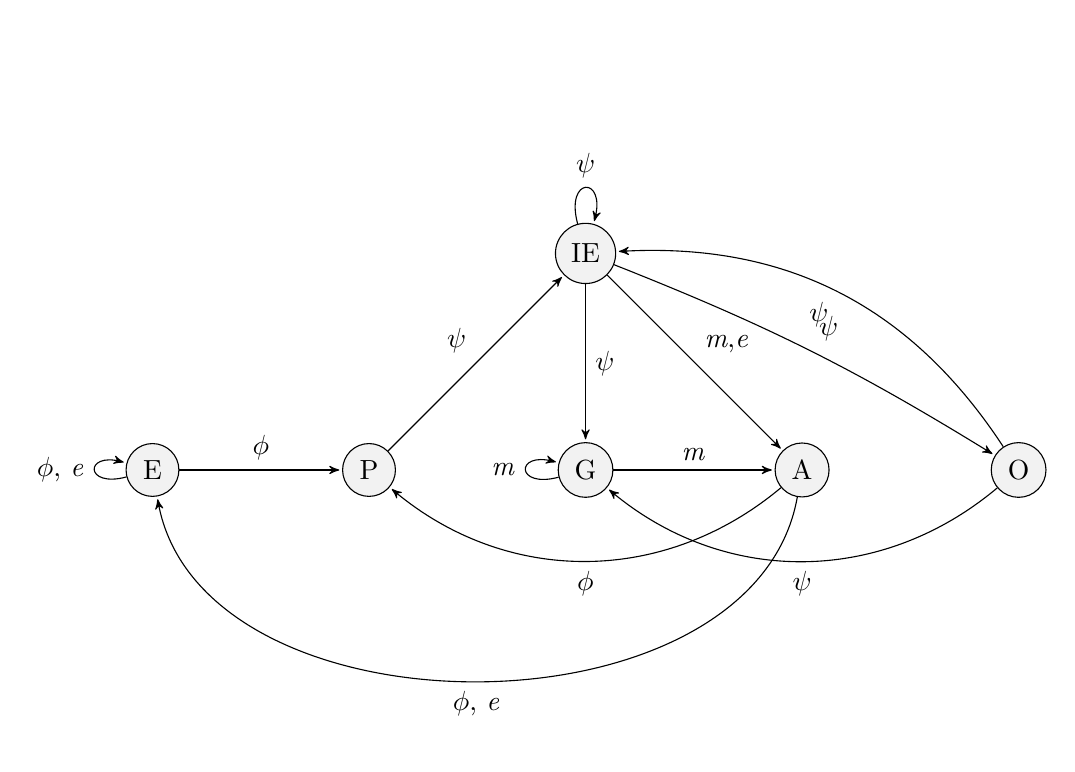
\begin{tikzpicture}[->,>=stealth',shorten >=1pt,auto,node distance=2.75cm]

  \node [invis] (i) [] {};
  \node[ball] (IE) [below of = i] {IE};
  \node[ball] (G) [below of = IE] {G};
  \node[ball] (A) [right of=G] {A};
  \node[ball] (O) [right of=A] {O};
  \node[ball] (P) [left of=G] {P};
  \node[ball] (E) [left of=P] {E};

  \path
    (IE) edge [loop above] node {$\psi$} (IE)
        edge [] node {$\psi$} (G)
        edge [] node {\textit{m},\textit{e}} (A)
        edge [bend left=5] node {$\psi$} (O)
    (O) edge [bend right = 30] node {$\psi$} (IE)
        edge [bend left = 40] node {$\psi$} (G)
    (A) edge [bend left = 40] node {$\phi$} (P)
        edge [bend left = 80] node {$\phi$, \textit{e}} (E)
    (P) edge [] node {$\psi$} (IE)
    (E) edge [loop left] node {$\phi$, \textit{e}} (E)
        edge [] node {$\phi$} (P)
    (G) edge [loop left] node {\textit{m}} (G)
        edge [] node {\textit{m}} (A);
    
\end{tikzpicture}
\end{figure}

The usefulness of this ontology is that it provides a single, simple, unifying language with which to describe a Fabula and, given that a Plot is a subset of a Fabula,  a Plot. It already suggests a digital representation as a graph-like data structure, and enriches the way of looking at a Plot as a whole, not only as a sequence of events, but rather as a sequence of \textit{causally related} events.

Also, the classification of story elements provided can be a first step towards their differentiation necessary to associate them with different methods of delivery to the audience (see section 1.1.3). The causal links can, instead, be useful for the generation of Discourse, by providing connectives between the description of related events.

The ways in which this model has been incorporated in the designing and construction of the Narration Engine will be described in the next chapters.

\pagebreak

\section{Propp's \textit{Morphology of the Folktale}}
Vladimir Propp's seminal work \textit{Morphology of the Folktale} \cite{propp} dates back to 1928. However it was largely ignored in the West until it was translated decades later. It is considered to be one of the most important works in the study of Folklore, as well as in the field of Morphology. 

Propp relies heavily on a large collection of folktales from traditional Russian folklore, \textit{Russian Fairy Tales}, composed by Aleksandr Afanas'ev and originally published in Russia in 1855. It is a collection of nearly 600 tales, which Propp uses as a dataset to base his analysis on.

\textit{Morphology of the Folktale} describes the results of a broad, systematic, scientific analysis of the structure of Russian folk tales. It focuses on the narrative structure of tales, and the classification of characters induced by their role in the story. Also it proposes an analysis of the Theme of folktales, they way in which they are combined together in tradition, and their intended meaning.

The work is broad and rather lengthy. Here, only the contents relevant to this work will be highlighted.

\bigskip

Propp notices how different characters in different tales often perform the same actions, to the point where in some case they might even be interchangeable without changing the general flow of the tale. This highlights the existence of a fixed structure within different tales, which would therefore contain recurring, constant elements. These elements are called \textit{Functions}. As a consequence of his analysis, Propp states that:

\begin{enumerate}\setlength{\itemsep}{0pt}
\item ``Functions of characters serve as stable, constant elements in a tale, independent of how and by whom they are fulfilled. They constitute the fundamental components of a tale."
\item ``The number of functions known to the fairy tale is limited."
\item ``The sequence of functions is always identical. "
\item ``All fairy tales are of one type in regard to their structure."
\end{enumerate}

This sequence of Functions then constitutes a constant skeleton, upon which every tale is constructed. They are defined as:

\begin{enumerate}\setlength{\itemsep}{0pt}
\setcounter{enumi}{-1}
\item Initial situation: not properly classified as a function, it is still part of every tale. In it the setting is presented, and some of the characters are briefly introduced.
\item \textit{Absentation}: One of the members of a family, or group, absents himself from home.
\item \textit{Interdiction}: The Hero is presented with an interdiction.
\item \textit{Violation}: The interdiction is violated.
\item \textit{Reconnaissance}: The Villain attempts to gather information. Information about the hero, his family, the location of an object and so on.
\item \textit{Delivery}: The Villain receives information
\item \textit{Trickery}: The villain attempts to deceive a victim. He or she tries to gain possession of the victim directly or of some of his/her belongings via trickery.
\item \textit{Complicity}: The victim unwillingly helps the Villain.
\item \textit{Villainy}: The Villain harms someone belonging to the community.
\item \textit{Lack}: One member of the community desires or lacks something.
\item \textit{Mediation}: The lack or misfortune is communicated to the Hero. He is commanded, requested or allowed to go, or simply presented with the problem.
\item \textit{Counteraction}: The Hero accepts or decides to act.
\item \textit{Departure}:  the Hero departs.
\item \textit{First Function of the Donor}: The Hero is tested, potentially allowing him to receive help in the form of a magical agent or a helping character. The test can take many forms, such as an attack, an interrogation, a request for help and so on.
\item \textit{Hero's Reaction}: The Hero reacts to the challenge posed to him by the Donor's test. He either fails or succeeds.
\item \textit{Receipt of a Magical Agent}: The Hero acquires the use of a magical agent. This can be an object a helpful creature.
\item \textit{Guidance}: The Hero is transported or led to the object of his search. Thanks to a variety of means.
\item \textit{Struggle}: Hero and Villain fight each other.
\item \textit{Branding}: The Hero is branded.
\item \textit{Victory}: The villain is defeated by the Hero.
\item \textit{Liquidation}: The original misfortune or lack is liquidated.
\item \textit{Return}: The Hero returns to his place of origin.
\item \textit{Pursued}:  A pursuer follows the Hero while he is returning.
\item \textit{Rescue}: The Hero escapes his pursuer.
\item \textit{Unrecognised arrival}: The Hero returns home, or reaches an other land, without being recognised.
\item \textit{Unfounded Claims}: A false hero poses as the hero to gain a prize in his place.
\item \textit{Difficult task}: The hero is presented with some kind of ordeal, or test.
\item \textit{Solution}: The test is resolved.
\item \textit{Recognition}: The hero's identity is confirmed.
\item \textit{Exposure}: The identity of the False Hero is confirmed. He is exposed as an impostor.
\item \textit{Transfiguration}: The Hero changes appearance. In some instances, the lifestyle of the Hero is changed instead.
\item \textit{Punisment}: The Villain is punished.
\item \textit{Marriage}: The Hero marries and / or ascends to the throne.

\end{enumerate}

Given the definition of these Functions, the author observes how they can be grouped in \textit{spheres of action}, groups in which certain characters,  or \textit{Dramatis personae}, how they are commonly defined in narratology, is always performing the action that is being recounted. Each Function has therefore a strong focus on one single specific \textit{dramatis persona}.

Seven spheres are identified, leading to the definition of seven distinct dramatis personae:

\begin{itemize}\setlength{\itemsep}{0pt}
\item \textit{Hero}: The main character of the tale, he departs on a quest to liquidate some lack, meets other characters, is tested, fights Villains and is often rewarded for defeating them.
\item \textit{Villain}: He who causes harm to someone, and is then sought after, fought and possibly defeated and punished.
\item \textit{Donor}: The Donor is the character who provides the hero with a magical agent.
\item \textit{Helper}: He transfers the Hero to its destination, helps him in the passing of a test, rescues him from pursuit or directly liquidates a lack.
\item \textit{Princess}: The person who is being sought for, often associated to her father or a similar figure, can assign tests, brand the hero, recognise him, punish villains and dispense rewards.
\item \textit{Dispatcher}: He who announces the lack or misfortune to the Hero, and dispatches him.
\item \textit{False Hero}: He claims the reward that should be justly given to the Hero, and is sometimes confronted, exposed and punished.
\end{itemize}

The strong claim presented here is that this classification of characters, and the character-function mapping is fixed and constant among all tales.

This allows for a very simple way of defining the skeleton of a story, by defining the functions that constitute it, and mapping the relevant characters to each of them.

\bigskip

An other interesting result described by Propp is that, not only characters are on the scene during the same group of functions in every tale, but also are introduced to the read in the same ways, and in the same moments.

\begin{itemize}\setlength{\itemsep}{0pt}
\item Hero, Princess and Dispatcher are always presented in the introductory scene.
\item The Donor is met accidentally by the Hero, while he is in his quest.
\item The Helper appears as a gift or reward to the Hero, after the passing of a test.
\item The Villain appears suddenly from outside, committing his villainy. He then disappears until the Hero has reached him.
\item The False Hero is sometimes introduced at the beginning of the tale, together with Hero, Princess and Dispatcher. Alternatively he is only made known when he claims the Hero's reward in his stead.
\end{itemize}

\bigskip

These are only a few of the results presented by Propp in his book, but are the ones that are more relevant to this work. They highlight a simple structure to a tale, almost rigid in its definition, which constitutes a very strong and useful base upon which to build a generation algorithm.

It is also important to note that these results come from the analysis of a dataset containing only tales from the traditional folklore of Russia. Russian folktales show particular promise in being used as a base for a Narration Engine, because they are particularly hero-centric, and therefore adapt well to a context in which a single user is at the center of the story.  

The ways in which these concepts have been used in the construction of the Engine are explained in the next chapters. 

\pagebreak

\chapter{A First Attempt}
An attempt was made at designing a generation algorithm based on the Fabula Model described in section 2.3. This path proved to be unfruitful.

\bigskip

The general procedure was to start from real-world tales, as the Fabula Model provides a way in which to deconstruct each of them into a network of story elements belonging to the ontology described by the model. 

Once a sufficient number of these networks was obtained, merging them together would have created a larger and more complex graph structure. Stories would have been generating by traversing this graph.

In this chapter are reported the details of this unsuccessful approach.

\pagebreak

\section{Tale Deconstruction}

The first step was the deconstruction process. This procedure was to be performed manually.

Each story event in the story was  to be translated into a \textit{Story Node} in the network, classified appropriately as an element of the ontology. Clearly, the classification of elements into six groups (Goals, Actions, Outcomes, Perceptions, Events and Internal elements) is not sufficient to capture the complexity of a story. A hierarchy of classes was devised to retain as much information as possible in the decomposition process, without needing an exceedingly large amount of them.

For example, Goal elements were further divided into three groups:

\begin{itemize}\setlength{\itemsep}{0pt}
\item \textit{AttainGoal}: the goal is to make a desired property true.
\item \textit{AvoidGoal}: the goal is to make a desired property false.
\item \textit{ObtainGoal}: the goal is to possess a certain item, or to hold a certain character captive.
\end{itemize}

Similar classification systems were used to further subdivide the other classes of elements in meaningful groups.

\bigskip

This required the design of a representation of a story State, so that properties of the current situation could be properly modeled. A system similar to that used within the STRIPS standard \cite{strips} was employed, representing a state as a collection of logic predicates, each of them expressing one property of the environment. Since this system is also part of the final architecture of the Narration Engine, it is explained in more detail in chapter 6.

This allowed for a more informative labeling of elements in the Fabula Network. Each node in the network carries a minimal description of an event, being its classification, as well as further specification in the form of one or more STRIPS predicates. 

\bigskip

A few examples of this translation are given here.

\begin{table}[H]
\caption{Decomposition of Story Events}
\label{tab:fabulanode}
\bigskip
\begin{tabular}{| l | l | l |}

\hline
Story Event & Node Classification & Specification Predicates \\
\hline
\textit{Little Red Riding Hood} & Internal: Desire & location(girl, grans\_house) \\
\textit{wanted to visit her gran...} & Goal: AttainGoal & location(girl, grans\_house)\\
\hline
\textit{Suddenly, the wolf} & Event & location(wolf, forest) \\
\textit{appeared beside her.} & & \\
\hline
\textit{Poor Granny did not have} & Action: HarmAction & captivity(wolf, gran), \\
\textit{time to say another word,} & &  harm(wolf, gran) \\
\textit{before the wolf}  & & \\
\textit{gobbled her up!}  & & \\ 
\hline
\textit{A few minutes later,} & Outcome: AttainPositive &  location(girl, grans\_house)\\
\textit{Little Red Riding Hood} & & \\
\textit{knocked on the door.}  & & \\
\hline
\textit{She realized that the} & Perception &  location(wolf, grans\_house)\\
\textit{person in the bed was} & & \\
\textit{not her Grandmother,}  & & \\
\textit{but a hungry wolf.}  & & \\
\hline
\end{tabular}
\end{table}

\bigskip

Given a few decomposed stories, the resulting networks were observed, considering the structure of the associated graphs. It was noted that:

\begin{itemize}\setlength{\itemsep}{0pt}
\item The resulting graph is akin to a simple, linear, path. 

This can be explained by observing the process which led to it: the Fabula associated to the tale can be seen as a connected graph, and a subset of its nodes is taken to define the Plot, as described in the Fabula Model (section 2.3). Then, the causality links force the order in which nodes have to be recounted, inducing a fixed ordering, as stated by Propp (section 2.4). Clearly, if links are induced by causality, and causality only propagates forward in time, there can be no loop.

Then the Plot is narrated, producing the text that was used for the decomposition. The decomposition task is performed following the order of the narrated story, and therefore replicates it in the resulting graph.

As a consequence, the final result is a connected graph describing a loopless sequence of events, following an ordering induced by causality.

\item There can be no branches that don't merge back into the main branch.

There can be branches merging into the main path of the story, but there can not be paths that branch out from it. Any outwards branching would necessarily have to merge back into the main one, or it would result in a loose end in the story: a chain of events that leads to nothing.

\end{itemize}

\bigskip

These properties are not true in general for any kind of narrative: in literature there are numerous examples in which events are not narrated following their causal ordering, and there can be loose ends to a story. There are even cases in which time is not considered to be entirely linear, possibly causing causality loops.

However, in the context of folktales generally adhering to Propp's model, the relative simplicity of the narrative structure makes these properties hold. The simplest way of recounting a story is in an ordered sequence of events, and this reflects on the shape of the resulting graph.

\bigskip

Below, the branching structure of a deconstructed tale is shown. The tale is Little Red Riding Hood, sourced from the \textit{Multilingual Folk Tale Database} \cite{mdb}.

Each dot does not represent a single story node, but rather a linear sequence of nodes, constituting a branch in the full network.

\begin{figure}[H]
\caption{Branching structure of Little Red Riding Hood}
 \label{fig:littlered}

\bigskip

\bigskip
 
 \centering
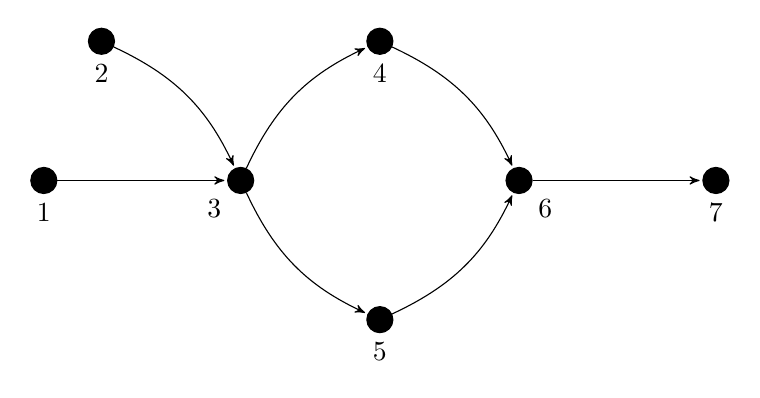
\begin{tikzpicture}[->,>=stealth',shorten >=1pt,auto,node distance=2.5cm]

\node[dot, name = 1,
label={[align=center]below:1}] (1) [] {};
\node[dot, name = 2, right of = 1,
label={[align=center]below left:3}] (2) [] {};
\node[dot, name = 3, above left of = 2,
label={[align=center]below:2}] (3) [] {};
\node[dot, name = 4, above right of = 2,
label={[align=center]below:4}] (4) [] {};
\node[dot, name = 5, below right of = 2,
label={[align=center]below:5}] (5) [] {};
\node[dot, name = 6, above right of = 5,
label={[align=center]below right:6}] (6) [] {};
\node[dot, name = 7, right of = 6,
label={[align=center]below:7}] (7) [] {};

\path
(1) edge [] node {} (2)
(3) edge [bend left = 20] node {} (2)
(2) edge [bend left = 20] node {} (4)
(2) edge [bend right = 20] node {} (5)
(4) edge [bend left = 20] node {} (6)
(5) edge [bend right = 20] node {} (6)
(6) edge [] node {} (7);


\end{tikzpicture}
\end{figure}

Each branch therefore represents a part of the whole story, as follows:

\begin{enumerate}\setlength{\itemsep}{0pt}
\item The main character, Little Red Riding Hood, is introduced, as well as her intentions to visit her grandmother. Her mother is also presented. Then, the girl departs from her home.
\item The Wolf is introduced.
\item The Wolf sees Little Red Riding Hood and approaches her, he asks about her, finds out what she is doing and leaves.
\item The Wolf runs to the grandmother's house through a shortcut, tricks her into opening the door, eats her and wears her clothes as disguise.
\item Little Red Riding Hood slowly reaches her grandmother's house, picking flowers along the way. 
\item Little Red Riding Hood sees the disguised Wolf and is suspicious about his appearance.
\item The Wolf attempts to eat her and she screams for help. A passing hunter intervenes, saving the girl and her grandmother, and killing The Wolf.
\end{enumerate}

\pagebreak

\section{Graph Merging and Issues}

Once a few stories were decomposed into sequence-like graphs, the next step was to merge them into a larger one. This was to be achieved by superimposing individual nodes respecting a certain definition of similarity. 

Given two graphs of story nodes, and given a definition of similarity between two nodes, it is certainly possible to identify pairs, or sets, of similar nodes and merge the two graphs, merging those nodes together. Repeating this for several stories, hence several sequences, would yield a large interconnected graph of story nodes.

\bigskip

An example of such procedure is shown here. Three stories, labelled \(A\), \(B\) and \(C\), have been decomposed into the three sequences \(a_1 ... a_8\), \(b_1 ... b_8\) and \(c_1 ... c_8\) . Two sets of nodes have been identified as similar: \(\{a_2,b_3\}\) and \(\{a_7,b_7,c_4\}\). 

\begin{figure}[H]
\caption{Plot sequences with node similarities}
 \label{fig:plotseq}
\centering
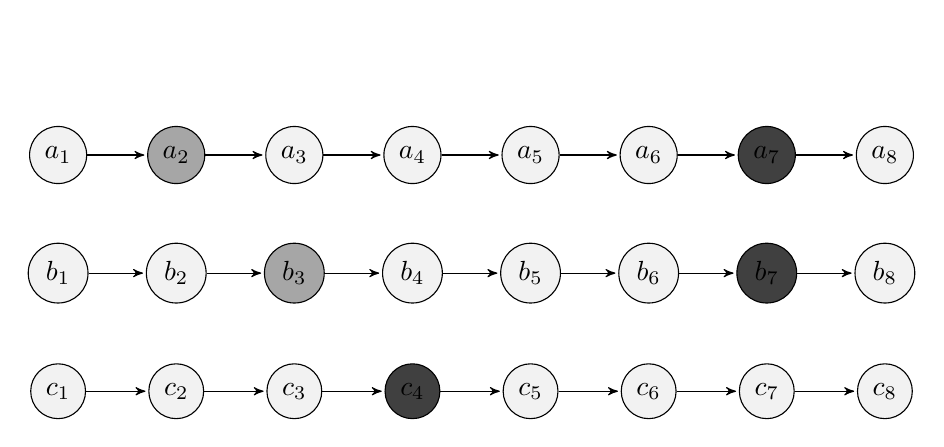
\begin{tikzpicture}[->,>=stealth',shorten >=1pt,auto,node distance=1.5cm]

\node[ball] (1a) [] {\(a_1\)};
\node[ball, fill=black!35] (2a) [right of = 1a] {\(a_2\)};
\node[ball] (3a) [right of = 2a] {\(a_3\)};
\node[ball] (4a) [right of = 3a] {\(a_4\)};
\node[ball] (5a) [right of = 4a] {\(a_5\)};
\node[ball] (6a) [right of = 5a] {\(a_6\)};
\node[ball, fill=black!75] (7a) [right of = 6a] {\(a_7\)};
\node[ball] (8a) [right of = 7a] {\(a_8\)};

\node[ball] (1b) [below of = 1a] {\(b_1\)};
\node[ball] (2b) [right of = 1b] {\(b_2\)};
\node[ball, fill=black!35] (3b) [right of = 2b] {\(b_3\)};
\node[ball] (4b) [right of = 3b] {\(b_4\)};
\node[ball] (5b) [right of = 4b] {\(b_5\)};
\node[ball] (6b) [right of = 5b] {\(b_6\)};
\node[ball, fill=black!75] (7b) [right of = 6b] {\(b_7\)};
\node[ball] (8b) [right of = 7b] {\(b_8\)};

\node[ball] (1c) [below of = 1b] {\(c_1\)};
\node[ball] (2c) [right of = 1c] {\(c_2\)};
\node[ball] (3c) [right of = 2c] {\(c_3\)};
\node[ball, fill=black!75] (4c) [right of = 3c] {\(c_4\)};
\node[ball] (5c) [right of = 4c] {\(c_5\)};
\node[ball] (6c) [right of = 5c] {\(c_6\)};
\node[ball] (7c) [right of = 6c] {\(c_7\)};
\node[ball] (8c) [right of = 7c] {\(c_8\)};

\node[invis] (i) [above of = 1a] {};


  \path
    (1a) edge [] node {} (2a)
    (2a) edge [] node {} (3a)
    (3a) edge [] node {} (4a)
    (4a) edge [] node {} (5a)
    (5a) edge [] node {} (6a)
    (6a) edge [] node {} (7a)
    (7a) edge [] node {} (8a)
    
    (1b) edge [] node {} (2b)
    (2b) edge [] node {} (3b)
    (3b) edge [] node {} (4b)
    (4b) edge [] node {} (5b)
    (5b) edge [] node {} (6b)
    (6b) edge [] node {} (7b)
    (7b) edge [] node {} (8b)
    
    (1c) edge [] node {} (2c)
    (2c) edge [] node {} (3c)
    (3c) edge [] node {} (4c)
    (4c) edge [] node {} (5c)
    (5c) edge [] node {} (6c)
    (6c) edge [] node {} (7c)
    (7c) edge [] node {} (8c);

\end{tikzpicture}
\end{figure}

The merging together of similar nodes would produce the following graph structure.

\begin{figure}[H]
\caption{Merged Plot Graph}
 \label{fig:fabulamodel}
\centering
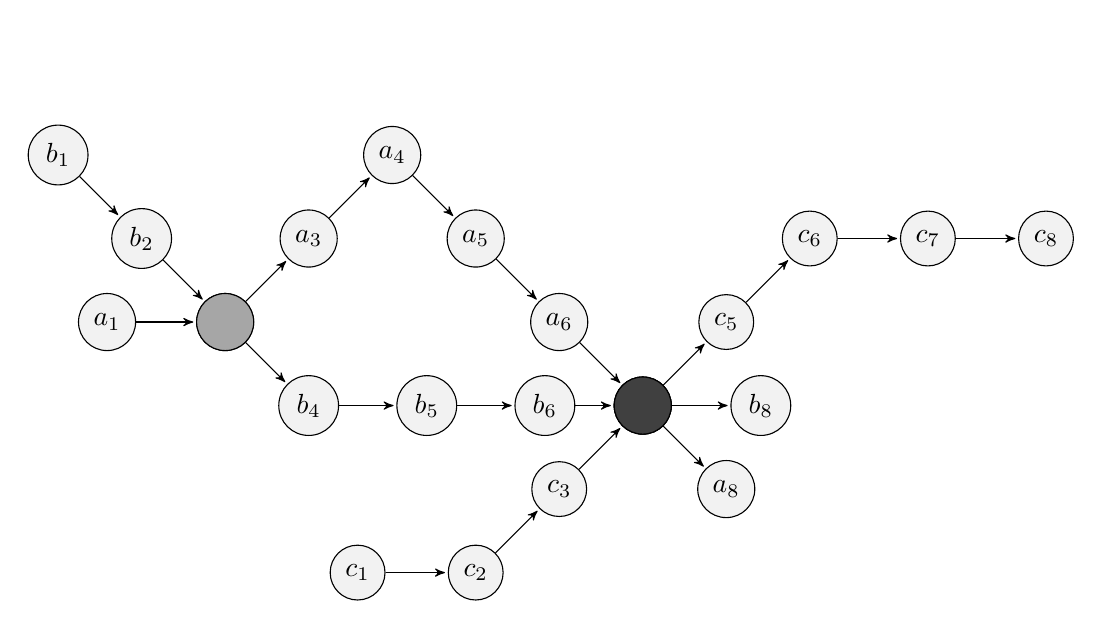
\begin{tikzpicture}[->,>=stealth',shorten >=1pt,auto,node distance=1.5cm]

\node[ball] (1a) [] {\(a_1\)};
\node[ball, fill=black!35] (2a) [right of = 1a] {\textcolor{black!35}{\(a_1\)}};
\node[ball] (3a) [above right of = 2a] {\(a_3\)};
\node[ball] (4a) [above right of = 3a] {\(a_4\)};
\node[ball] (5a) [below right of = 4a] {\(a_5\)};
\node[ball] (6a) [below right of = 5a] {\(a_6\)};
\node[ball, fill=black!75] (7a) [below right of = 6a] {\textcolor{black!75}{\(a_1\)}};
\node[ball] (8a) [below right of = 7a] {\(a_8\)};

\node[ball, fill=black!35] (3b) [right of = 1a] {\textcolor{black!35}{\(a_1\)}};
\node[ball] (2b) [above left of = 3b] {\(b_2\)};
\node[ball] (1b) [above left of = 2b] {\(b_1\)};
\node[ball] (4b) [below right of = 3b] {\(b_4\)};
\node[ball] (5b) [right of = 4b] {\(b_5\)};
\node[ball] (6b) [right of = 5b] {\(b_6\)};
\node[ball, fill=black!75] (7b) [below right of = 6a] {\textcolor{black!75}{\(a_1\)}};
\node[ball] (8b) [right of = 7b] {\(b_8\)};

\node[ball, fill=black!75] (4c) [below right of = 6a] {\textcolor{black!75}{\(a_1\)}};
\node[ball] (3c) [below left of = 4c] {\(c_3\)};
\node[ball] (2c) [below left of = 3c] {\(c_2\)};
\node[ball] (1c) [left of = 2c] {\(c_1\)};
\node[ball] (5c) [above right of = 4c] {\(c_5\)};
\node[ball] (6c) [above right of = 5c] {\(c_6\)};
\node[ball] (7c) [right of = 6c] {\(c_7\)};
\node[ball] (8c) [right of = 7c] {\(c_8\)};

\node[invis] (i) [above of = 1b] {};


  \path
    (1a) edge [] node {} (2a)
    (2a) edge [] node {} (3a)
    (3a) edge [] node {} (4a)
    (4a) edge [] node {} (5a)
    (5a) edge [] node {} (6a)
    (6a) edge [] node {} (7a)
    (7a) edge [] node {} (8a)
    
    (1b) edge [] node {} (2b)
    (2b) edge [] node {} (3b)
    (3b) edge [] node {} (4b)
    (4b) edge [] node {} (5b)
    (5b) edge [] node {} (6b)
    (6b) edge [] node {} (7b)
    (7b) edge [] node {} (8b)
    
    (1c) edge [] node {} (2c)
    (2c) edge [] node {} (3c)
    (3c) edge [] node {} (4c)
    (4c) edge [] node {} (5c)
    (5c) edge [] node {} (6c)
    (6c) edge [] node {} (7c)
    (7c) edge [] node {} (8c);

\end{tikzpicture}
\end{figure}

A graph like this could be explored in multiple ways, starting from the beginning of any story sequence and ending at any story end. 

Nodes that have been merged would act as choice points between the following of different story sequences, while the exploration policy would determine which stories are included in the final path. An example of such exploration path, on the graph shown above, would be described by the sequence \(b_1...b_3,a_3...a_7,c_5...c_8\).

The output of an exploration process would be a sequence of story nodes, constituting a new story. This new story would be a mix of real-world ones intertwined together. 

\bigskip

The adherence to constraints could be observed by pre-processing story sequences prior to the merging, extracting the necessary information and storing them into an appropriate data structure which would be, in turn, used during the exploration process to determine which story is to be followed next.

\bigskip

The exploration of this graph, and the subsequent output of the corresponding exploration path, would have resulted in a new sequence of story nodes and therefore in a new story, as mix of pre-existing real world ones.

\bigskip

This system was not fully developed nor fully tested. A few stories were decomposed into story node sequences, but then such problems emerged that it became clear that this approach would have proved unsuccessful. These problems have to do with two phases of the process: the phase in which real-world tales are decomposed, and the phase in which the resulting structures are merged together.

\begin{itemize}\setlength{\itemsep}{0pt}
\item \textbf{Decomposition Phase}: in order to function effectively, the system needs to be primed with a sufficient number of decomposed tales. The more tales are available, the more varied the output will be, since the graph on which the exploration is performed would grow accordingly. Too small a number of available tales would cause the output to be extremely uniform.

\bigskip

the decomposition of a tale into a sequence of story nodes proved to be an extremely intricate task: it required a sequence of complex operations to be performed on each sentence in the original tale:

\begin{enumerate}\setlength{\itemsep}{0pt}
\item Each sentence has to be carefully analysed to determine its full meaning. 
\item Such meaning has to be then decomposed into individual nodes. 
\item Each one of these nodes has to be classified following a complex hierarchical system, in order to preserve the relative information. 
\item The type of causal link between each pair of nodes has to be determined. In some cases there is only one possible causality type, as from the original Fabula Model, while in other cases a choice must be taken between a few alternatives.
\item The whole result has to be fed into a computer so that it can be processed.
\end{enumerate}

It is immediate that this process is extremely time consuming, and single person would require an exceedingly long time to decomposed a suitable number of stories. Involving multiple people to collaborate in this process was not possible in the context of this work, and it would have introduced new problems in the training of these collaborators, and the necessity of maintaining a certain uniformity in the classification, since personal interpretation is part of the task.

In literature, a few attempts have been made at automating the decomposition of narrative, one of which, based on a mix of Hidden Markov Models and Latent Semantic Analysis, was examined, since it was specifically designed to work on Russian folktales in the context of Propp's model \cite{autopropp}. However, the system did not meet the required level of accuracy in the decomposition, since it only focused on recognising Propp Functions.

\bigskip

An other issue with the decomposition process was the fine tuning of the level of accuracy of the node classification. As new stories were incorporated, lacks in the existing classification system were made evident, requiring the addition of new classes or new predicate types to correctly represent the new information. This in turn caused an explosion in the amount of classes to be used, which made the classification task even more demanding.

\item \textbf{Merging Phase}: the merging of story sequences consisted in the merging of some of their story nodes. Every time two nodes are merged together, a new choice point is induced in the general graph. 

In order to have an effective system, it is necessary to generate a suitable number of these points: unless enough choices are available, the exploration process will necessarily proceed along the path of one of the original stories, without generating anything different.

The merging, or lack thereof, of story nodes depends upon a definition of the property of similarity between nodes, based on their representation.

Each node, as shown in table 2.1, is represented as a pair:\\ 
\(<Classification, Specification>\), where \(Classification\) consists in a node type and optionally a node subtype, while \(Specification\) in a set of logic predicates.

Different definitions of the property were attempted: the loosest of which being a simple confrontation of type and subtype. Stricter definitions applied different logic unification models to the Specification predicates, even involving a classification of characters following Propps' model.

No definition proved to be broad enough to produce a sufficient number of choice points, while also being strict enough to preserve coherence. It is possible that, given a sufficient number of stories, it would have been easier to design an effective similarity function but, as explained above, the amount of available stories was severely limited.

\bigskip

An explanation of such difficulty in finding similar story nodes can be searched in the process that brought these centuries-old pieces of narrative to us. 

These tales emerged from a long process of oral transmission from person to person. During this process, multiple variants of each tale emerged, and different tales were sometimes mixed together, re-elaborated, truncated. This would seem to imply the coexistence of many similar stories, caused by this chaotic process of "collaborative writing" among multiple authors and multiple generations. This would in turn imply the existence of many similar nodes belonging to similar tales.

However, between the 19th and the early 20th century, the main systemic collection works of these, previously orally transmitted, stories were published. Notable examples include \textit{Kinder- und Hausmärchen} by the Grimm brothers (1812), and the already cited work by Aleksandr Afanas'ev (1855).

In these large collections, sets of similar tales were "collapsed" together into a single version \cite{propp}, thereby filtering out most of the variants to a single theme. These collections form the basis of most folktale datasets, including those used in this work. 

\bigskip

This might explain why it was difficult to find stories with a high degree of similarity: because most of them didn't survive the filtering process necessary in the gathering of a large amount of them in large collections.
\end{itemize}

\bigskip

Once this approach proved to be ineffective, an other was attempted, which instead led to the design of a working, albeit simple, system. This will be the subject of the next chapters.

\pagebreak

\chapter{General Architecture}
This chapter will be an overview of the general architecture of the system. Structure and function of the various elements involved will be explained more in depth in the next chapters. 

\bigskip

This system, once developed further, is to be used to reinforce the engagement of users in a set of activities that will be proposed to them, by encasing a group of them in a narrative structure.

This requires it to produce a meaningful story and associate some of its elements to activities, specified prior to the generation.

The final output will be in the form of a .json file, carrying a mapping between pieces of texts and activities to be proposed to the user, where the activity is null for all those text pieces that are not associated to anything.

\bigskip

Before any generation can take place, the system has to be correctly initialised and configured. The operation of providing each module with the appropriate parameters will be explained along with the corresponding module.

In particular, one of the parameters required is the set of activities that are to be part of the output. The story output will necessarily contain them.

\bigskip

Once the system is ready and all parameters are set, a Plot Generation layer (chapter 4) defines a Plot, as a sequence of Story Nodes similar to those described in the last chapter. 

\bigskip

The inner workings of this layer borrow elements from both Propp's model and the Fabula Model. A sequence of Propp Functions is composed, based on an algorithm that follows a set of pre composed Plots, while recursively introducing new subplots to overcome obstacles in case they arise.

In parallel, within each Function, the ways in which that scene can develop are defined through a probabilistic graph structure. Nodes within these structures are defined according to the Fabula Mode and represent atomic story events. 

A graph search algorithm then traverses the graph outputting a sequence of nodes that constitute the specific chain of events that make up the corresponding scene.

\bigskip

At both these levels of abstraction, the adherence to generation constraints and coherence rules are ensured through the interaction with a structure describing the State of the generation. This module is implemented employing the STRIPS standard, and it will explained further in section 5.2.1.

\begin{figure}[H]
\caption{Architecture of the Plot Generation Layer}
 \label{fig:plotgen}
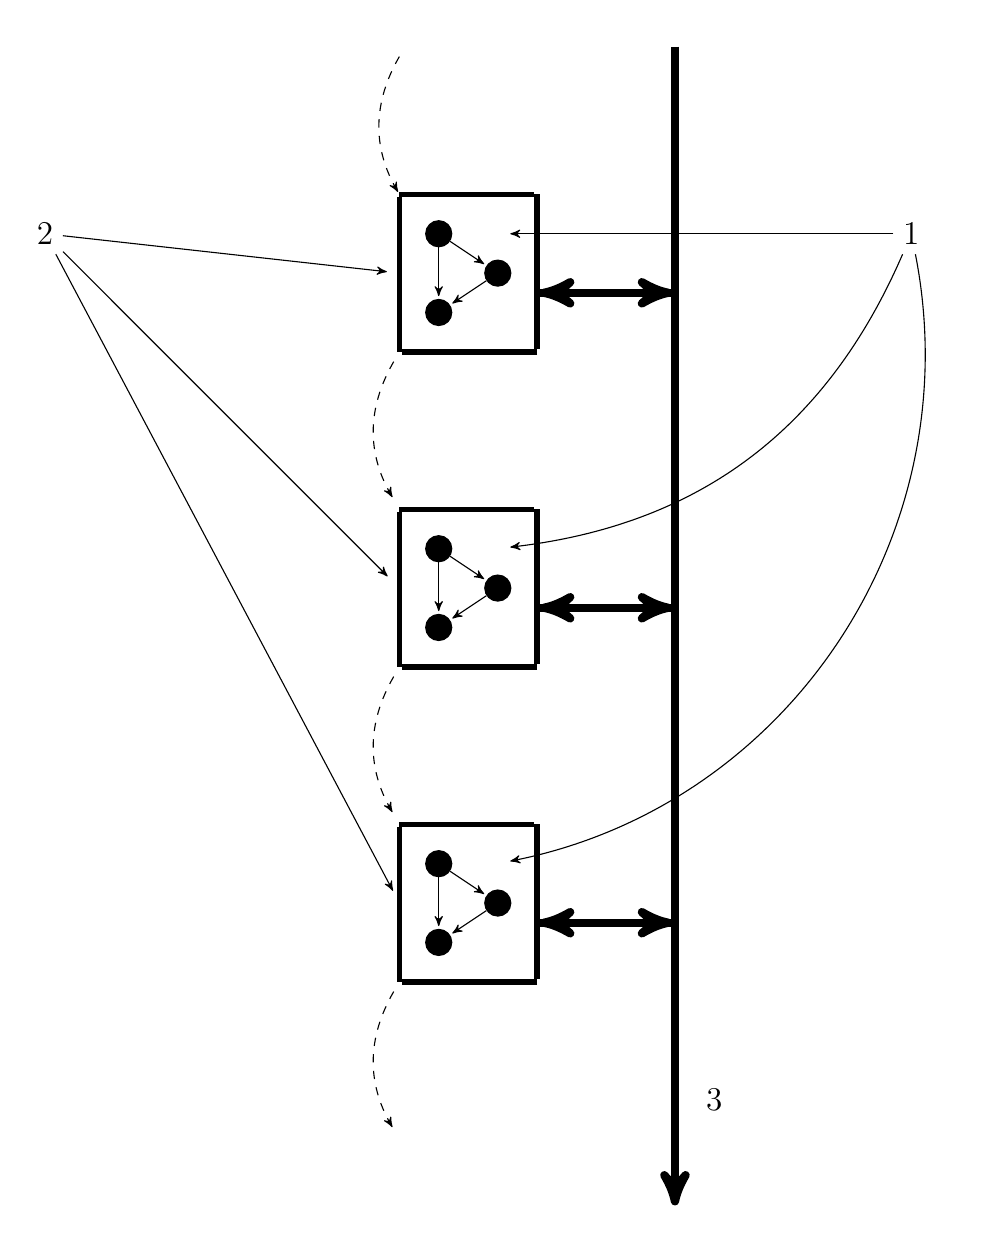
\begin{tikzpicture}[->,>=stealth',shorten >=1pt,auto,node distance=2.75cm]

    \node[dot] at (0,0) (a1) [] {};
    \node[dot] at (0.75,-0.5) (a2) [] {};
    \node[dot] at (0,-1) (a3) [] {};
    
    \path
    (a1) edge [] node {} (a2)
    (a1) edge [] node {} (a3)
    (a2) edge [] node {} (a3);
      
    \node[invis] at (-0.5,-1.5) (ai4) [] {};
 
    \path
    (-0.5,0.5) edge [-, line width=2] node {} (1.25,0.5)
    (1.25,0.5) edge [-, line width=2] node {} (1.25,-1.5)
    (1.25,-1.5) edge [-, line width=2] node {} (-0.5,-1.5)
    (-0.5,-1.5) edge [-, line width=2] node {} (-0.5,0.5);
    
    %=====================
    
    \node[dot] at (0,-4) (b1) [] {};
    \node[dot] at (0.75,-4.5) (b2) [] {};
    \node[dot] at (0,-5) (b3) [] {};
      
    \node[invis] at (-0.5,-3.5) (bi1) [] {};
    \node[invis] at (-0.5,-5.5) (bi4) [] {};
  
    \path
    (b1) edge [] node {} (b2)
    (b1) edge [] node {} (b3)
    (b2) edge [] node {} (b3);
    
    \path
    (-0.5,-3.5) edge [-, line width=2] node {} (1.25,-3.5)
    (1.25,-3.5) edge [-, line width=2] node {} (1.25,-5.5)
    (1.25,-5.5) edge [-, line width=2] node {} (-0.5,-5.5)
    (-0.5,-5.5) edge [-, line width=2] node {} (-0.5,-3.5);
    
 %=====================
    
    \node[dot] at (0,-8) (c1) [] {};
    \node[dot] at (0.75,-8.5) (c2) [] {};
    \node[dot] at (0,-9) (c3) [] {};
      
    \node[invis] at (-0.5,-7.5) (ci1) [] {};
    \node[invis] at (-0.5,-9.5) (ci4) [] {};
  
    \path
    (c1) edge [] node {} (c2)
    (c1) edge [] node {} (c3)
    (c2) edge [] node {} (c3);
    
    \path
    (-0.5,-7.5) edge [-, line width=2] node {} (1.25,-7.5)
    (1.25,-7.5) edge [-, line width=2] node {} (1.25,-9.5)
    (1.25,-9.5) edge [-, line width=2] node {} (-0.5,-9.5)
    (-0.5,-9.5) edge [-, line width=2] node {} (-0.5,-7.5);
    
    \node [invis] at (-0.5,-11.5) (di1) [] {};
    \path
    (bi4) edge [dashed, bend right = 30] node {} (ci1)
    (ai4) edge [dashed, bend right = 30] node {} (bi1)
    (ci4) edge [dashed, bend right = 30] node {} (di1);
    
    \node[invis] at (0.75,0) (ae11) [] {};
    \node[invis] at (0.75,-4) (ae12) [] {};
    \node[invis] at (0.75,-8) (ae13) [] {};
    \node[invis] at (6,0) (as1) [] {\large1};
    
    \path
    (as1) edge [] node {} (ae11)
    (as1) edge [bend left = 30] node {} (ae12)
    (as1) edge [bend left = 45] node {} (ae13);
    
    \node[invis] at (-5,0) (as2) [] {\large2};
    
    \node[invis] at (-0.5,-0.5) (ae21) [] {};
    \node[invis] at (-0.5,-4.5) (ae22) [] {};
    \node[invis] at (-0.5,-8.5) (ae23) [] {};
    
    \path 
    (as2) edge [] node {} (ae21)
    (as2) edge [] node {} (ae22) 
    (as2) edge [] node {} (ae23); 
    
    \node[invis] at (3,2.5) (s1) [] {};
    \node[invis] at (3,-12.5) (s2) [] {};
    
    \path
    (1.25,-0.75) edge [line width = 3] node {} (3,-0.75)
    (3,-0.75) edge [line width = 3] node {} (1.25,-0.75)
    (1.25,-4.75) edge [line width = 3] node {} (3,-4.75)
    (3,-4.75) edge [line width = 3] node {} (1.25,-4.75)
    (1.25,-8.75) edge [line width = 3] node {} (3,-8.75)
    (3,-8.75) edge [line width = 3] node {} (1.25,-8.75)
    (s1) edge [line width = 3] node {} (s2);
    
    \path
    (-0.5,2.25) edge [dashed, bend right =30] node {} (-0.5,0.5);
    
    \node[invis] at (3.5,-11) (s) [] {\large3};
  
\end{tikzpicture}
\end{figure}

\begin{enumerate}\setlength{\itemsep}{0pt}
\item Probabilistic graphs serve as model of the possible sequences of events that constitute a scene/function. Traversing one of these graphs gives out a sequence of nodes that describes the developing of the scene.
\item Functions are chained together following recursive rules based on plots and subplots. The concatenation of the corresponding node sequences is what constitutes the final plot.
\item Both components interact with a State that propagates forward during the generation process, used to ensure adherence to constraints.
\end{enumerate}

\bigskip

At the end of this process, a Plot is given in output, as a sequence of story nodes. This is going to be input for the second layer, that focuses on translating this plot into readable text.

This component iteratively parses the plot, associating nodes to variables, and variables to text and activities, using a set of dictionaries to process variables into appropriate, consistent, ground expressions. This process will be the subject of chapter 5.

\bigskip

Here is shown a schematic of the general architecture.

\begin{figure}[H]
\caption{General Architecture}
 \label{fig:generalarchitecture}
 \bigskip
 \bigskip
\centering
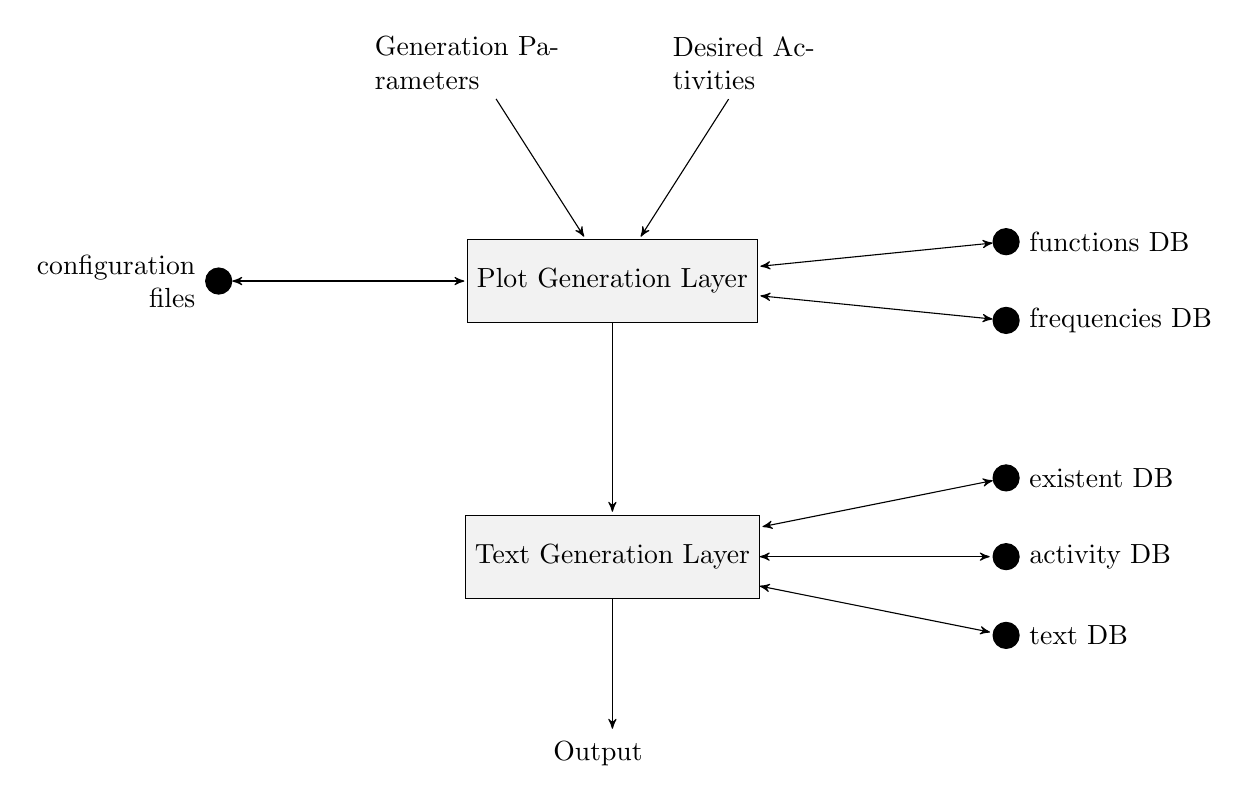
\begin{tikzpicture}[->,>=stealth',shorten >=1pt,auto,node distance=2.5cm]

    \node [block, minimum height=3em, name = l1] {Plot Generation Layer};
    \node [block, below of = l1, minimum height=3em, yshift = -1cm, name = l2] {Text Generation Layer};
    
    \node [invis, above left of = l1, text width = 2.5cm, yshift = 1cm, name=gen] {Generation Parameters};
    \node [invis, above right of = l1, text width = 2cm, yshift = 1cm, name=act] {Desired Activities};
    
    \node [dot, left of = l1, xshift = -2.5cm, 
    label={[align=right]left:configuration\\files}, name = cfg] {};
    
    \node [dot, right of = l1, xshift = 2.5cm, yshift=-0.5cm,
    label={[align=right]right:frequencies DB}, name = freq] {};
    \node [dot, right of = l1, xshift = 2.5cm, yshift = 0.5cm,
    label={[align=right]right:functions DB}, name = fun] {};

    \node [dot, right of = l2, xshift = 2.5cm, yshift = 1cm,
    label={[align=right]right:existent DB}, name = exi] {};   
    \node [dot, right of = l2, xshift = 2.5cm, yshift = 0cm,
    label={[align=right]right:activity DB}, name = acti] {};
    \node [dot, right of = l2, xshift = 2.5cm, yshift = -1cm,
    label={[align=right]right:text DB}, name = tex] {};
    
    \node [invis, below of = l2, text width = 1.5cm, name = out] {Output};
    
    \draw [->] (gen) -- node[] {} (l1);
    \draw [->] (act) -- node[] {} (l1);
    \draw [<->] (cfg) -- node[] {} (l1);
    \draw [<->] (fun) -- node[] {} (l1);
    \draw [<->] (freq) -- node[] {} (l1);
    \draw [<->] (exi) -- node[] {} (l2);
    \draw [->] (l1) -- node[] {} (l2);
    \draw [<->] (l2) -- node[] {} (acti);
    \draw [<->] (l2) -- node[] {} (tex);
    \draw [->] (l2) -- node[] {} (out);

\end{tikzpicture}
\end{figure}

A set of database files is used by both layers of the architecture: they constitute a knowledge base, containing data necessary to the process, as well as containing information regarding past activities of the system. Their function will be described in the next chapters, along with the inner workings of the relative generation layer.

\bigskip

The final output is a .json file: a sequence of triplets, each containing: a node identifier, e small piece of readable text and, when such association is possible, an identifier to an activity to be proposed to the user. This structure can then be used to compose a story interweaved with user activities, delivered by whatever media are available.

\pagebreak

\chapter{Plot Generation}
The subject of this chapter is the first layer in the generation architecture. This component generates a Plot, given a set of user-defined parameters and the proper knowledge base.

\section{Scenes as Propp Functions}
The Plot Generation process is based on the concept of Function, as defined by Propp (section 2.4). Each function can be seen as a scene in the story: each one of these scenes can develop in different ways. Propp already gives, for each function, the different ways in which that function has been carried out in the dataset he used.

\subsection{Modelling a Function}
Each Function/scene is modeled as a probabilistic graph, in which different paths correspond to different ways in which the scene can progress. Nodes in these graphs are defined following the Fabula Model explained in section 2.3, similarly to the nodes used in the deconstruction of tales explained above.

The difference between these nodes and those explained before lies in the fact that these follow a simplified ontology. In the failed attempt at story generation explained in the previous chapters nodes were used to capture the semantic structure of a given tale. 

In the original work in which the model was proposed they were being used for character simulation. In this case, however, nodes are not required to carry any semantic information, which will be provided later by an association with text.

As a consequence the nodes used contain simpler information, being the pair\\ \(<label,classification>\). The \(classification\) variable identifies a class in a simplified version of the Fabula Network Model. The original model defined six classes: Actions, Goals, Perceptions, Outcomes, Internal Elements and Events. The classes Perceptions and Internal Elements have been grouped together in the Perception-Internal class. This was possible because the distinction between the two was aimed at providing a simulation step in the internal process of reasoning of a character. Given that this is no longer being done, the distinction became redundant.

The resulting data structure borrows from both Propp's model and the Fabula Model: a graph of nodes based on the ontology given within the latter constitutes one of the elements (a Function) described in the first.

\bigskip

Following this model, the 31 Functions described by Propp have been grouped together into 17 graph structures, each one describing a scene. An example is given here in the form of the \textit{FirstFunction-Reaction} Function, which groups together two of Propp's: \textit{First Function of the Donor}, and \textit{Hero's Reaction}. In this, the Hero meets the Donor and performs some kind of test.

\bigskip

In the figure, black dots represent a single node with its label, while nodes \(A\) to \(G\) represent longer, linear paths comprising multiple nodes. Each of these corresponds to one of the possible developments of the scene as defined by Propp, as follows:

\begin{itemize}\setlength{\itemsep}{0pt}
\item \textbf{A}: the test consists in a difficult task to be performed by the Hero.
\item \textbf{B}: a test of knowledge. The Donor interrogates the Hero.
\item \textbf{C}: the Hero finds the Donor to be prisoner of someone else. The testing lies in whether he frees him or not. 
\item \textbf{D}: the Hero captures the Donor. He asks for mercy.
\item \textbf{E}: the Donor attacks the hero without provocation. The hero "passes" the test if he emerges victorious.
\item \textbf{F}: the Donor offers the Hero an exchange, or a trade.
\item \textbf{G}: the Donor is in need of help, the Hero may or may not intervene.
\end{itemize}

\begin{figure}[H]
\caption{Structure of a Propp Function}
 \label{fig:proppfunction}
 
 \bigskip
 
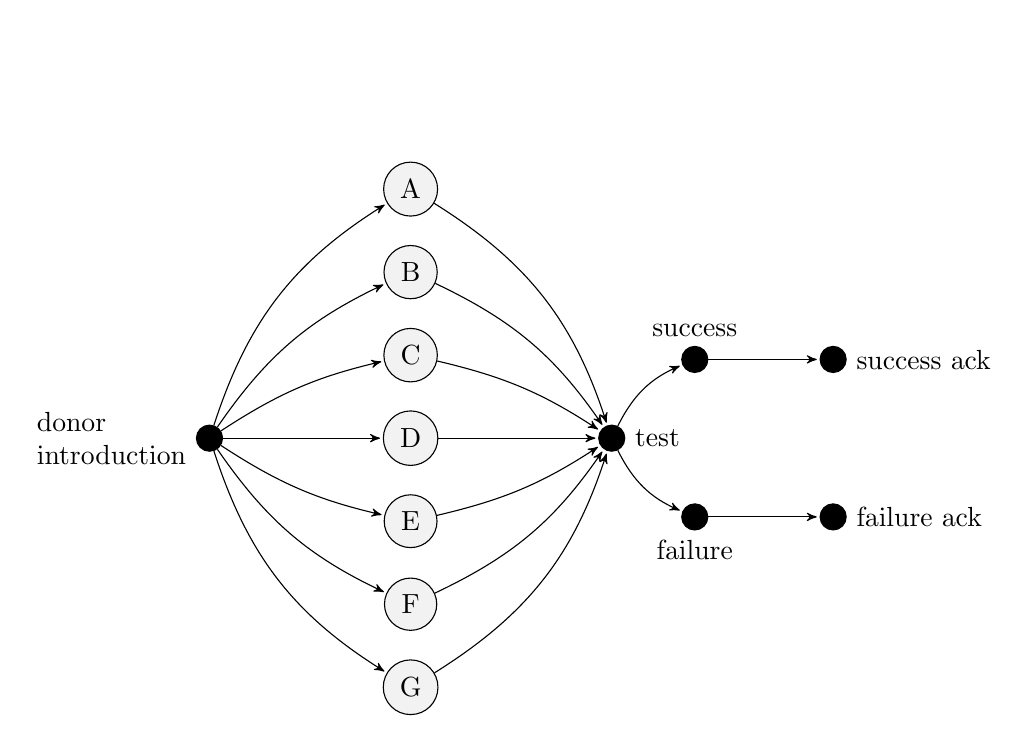
\begin{tikzpicture}[->,>=stealth',shorten >=1pt,auto,node distance=30]

%\node [invis, text width = 2cm, name = intro] {donor\\introduction};
\node[dot,label={[align=left]left:{donor\\introduction}}] (intro) [] {};
\node[ball] (D) [right of = intro, xshift = 1.5cm] {D};
\node[ball] (C) [above of = D] {C};
\node[ball] (B) [above of = C] {B};
\node[ball] (A) [above of = B] {A};
\node[ball] (E) [below of = D] {E};
\node[ball] (F) [below of = E] {F};
\node[ball] (G) [below of = F] {G};
\node[dot,label={[align=left]right:{test}},
right of = D, xshift = 1.5cm] (test) [] {};
\node[dot,label={[align=left]above:{success}},
right of = test, yshift = 1cm] (success) [] {};
\node[dot,label={[align=left]below:{failure}},
right of = test, yshift = -1cm] (failure) [] {};
\node[dot,label={[align=left]right:{success ack}},
right of = success, xshift = 20] (success_ack) [] {};
\node[dot,label={[align=left]right:{failure ack}},
right of = failure, xshift = 20] (failure_ack) [] {};
\node[invis] (i) [above of = A, yshift = 25] {};

\path
(intro) edge [bend left = 20] node {} (A)
(intro) edge [bend left = 15] node {} (B)
(intro) edge [bend left = 10] node {} (C)
(intro) edge [] node {} (D)
(intro) edge [bend right = 10] node {} (E)
(intro) edge [bend right = 15] node {} (F)
(intro) edge [bend right = 20] node {} (G)
(A) edge [bend left = 20] node {} (test)
(B) edge [bend left = 15] node {} (test)
(C) edge [bend left = 10] node {} (test)
(D) edge [] node {} (test)
(E) edge [bend right = 10] node {} (test)
(F) edge [bend right = 15] node {} (test)
(G) edge [bend right = 20] node {} (test)
(test) edge [bend left = 20] node {} (success)
(test) edge [bend right = 20] node {} (failure)
(success) edge [] node {} (success_ack)
(failure) edge [] node {} (failure_ack);


\end{tikzpicture}
\end{figure} 

An example of a complete path on this graph, passing through the sequence \(C\) is given below. For each node a brief interpretation is given for readability. This is not part of the real data structure.

\begin{table}[H]
\caption{Node in a Scene Path}
\label{tab:scenewalk}
\bigskip
\begin{tabular}{| l | l | l |}

\hline
Label & Classification & Interpretation \\
\hline
donor\_introduciton & Event & the Donor character is introduced \\
prisoner\_ack & Perception/Internal & the Donor perceives the Hero \\
desire\_freedom & Goal & the Donor wants to be free \\
freedom\_request & Action & the Donor asks the Hero for help \\
request\_ack & Perception/Internal & the Hero receives the request \\
test & Action & the Hero is subjected to the test \\
 &  & (in this case freeing the Donor) \\
success & Outcome & the Hero is successful \\
success\_ack & Perception/Internal & the Donor acknoweledges the result\\
\hline

\end{tabular}
\end{table}

\bigskip

\subsection{Graph Traversal and Constraints}
Given a properly defined graph structure, some nodes can be defined as "initial" nodes if they have an indegree of 0. Specularly, nodes with outdegree 0 are considered "final". 

The generation of a scene sequence involves the finding of a path, connecting an initial node to a final one.

Still, not all paths from an initial node to a final one are necessarily valid: depending on how the graph was defined, there might be cases in which integrity constraints make a path not valid. For instance, in the \textit{Struggle - Branding} Function, in which the Hero fights the Villain, one of the possible outcomes is that the Hero acquires an item previously in possession of the Villain. Any path in which the hero is defeated cannot therefore contain the node (or nodes) in which the Hero acquires said item.

\bigskip

A system is in place to support the introduction of constraints concerning the "validity" of paths: each node can optionally be associated with logic preconditions that define whether it can be included in the scene path or not. Since this system is more intensely used in the concatenation of different scenes it will be explained in the next sections.

The generation of a valid path is performed via a standard graph exploration algorithm. The graph is traversed Depth-First: at each step the preconditions of all successors to the current node are evaluated, and only those for which they are satisfied are considered in the exploration.

This effectively equals to performing the same traversal algorithm on a graph from which invalid nodes are removed completely. The output is then guaranteed not to contain any of them, therefore only producing valid paths.

\bigskip

The disabling of nodes based on logic conditions is not the only available mechanic to impose constraints on the generation of a scene. A system is in place that allows for the specification of nodes that must be part of the final path. 

This set of nodes must be specified before the exploration process begins. The operation of making the presence of a node mandatory is given the name of \textit{Injection}.

Injections are implemented by exploiting a property of the Depth-First search algorithm used to traverse the graph: if a "dead end" is reached, the process backtracks to the last choice point available.

Therefore, whenever the exploration process reaches a final node, instead of it terminating immediately, the current reverse path to the initial node is evaluated. If it is found to contain all the injected nodes, the process terminates. Otherwise it backtracks and continues.

\bigskip

\begin{figure}[H]
\caption{Backtracking in DFS search}
 \label{fig:backtracking}
 
 \bigskip
 \bigskip

\begin{minipage}[c]{0.5\textwidth}
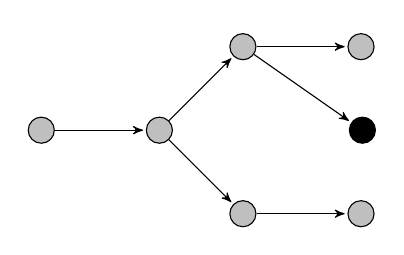
\begin{tikzpicture}[->,>=stealth',shorten >=1pt,auto,node distance=1.5cm]

\node[dot, fill = black!25] (1) [] {};
\node[dot, fill = black!25, right of = 1] (2) [] {};
\node[dot, fill = black!25, below right of = 2] (3) [] {};
\node[dot, fill = black!25, right of = 3] (4) [] {};
\node[dot, fill = black!25, above right of =2] (5) [] {};
\node[dot, fill = black, below right of =5, xshift = 13] (6) [] {};
\node[dot, fill = black!25, right of =5] (7) [] {};

\path
(1) edge [] node {} (2)
(2) edge [] node {} (3)
(3) edge [] node {} (4)
(2) edge [] node {} (5)
(5) edge [] node {} (6)
(5) edge [] node {} (7);
\end{tikzpicture}
\end{minipage}
\begin{minipage}[c]{0.5\textwidth}
This is the graph associated to a Function. A node has been injected (in black) and must necessarily appear in the final path.
\end{minipage}
\end{figure}

\bigskip

\begin{minipage}[c]{0.5\textwidth}
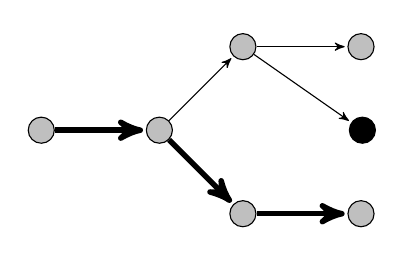
\begin{tikzpicture}[->,>=stealth',shorten >=1pt,auto,node distance=1.5cm]

\node[dot, fill = black!25] (1) [] {};
\node[dot, fill = black!25, right of = 1] (2) [] {};
\node[dot, fill = black!25, below right of = 2] (3) [] {};
\node[dot, fill = black!25, right of = 3] (4) [] {};
\node[dot, fill = black!25, above right of =2] (5) [] {};
\node[dot, fill = black, below right of =5, xshift = 13] (6) [] {};
\node[dot, fill = black!25, right of =5] (7) [] {};

\path
(1) edge [line width = 2] node {} (2)
(2) edge [line width = 2] node {} (3)
(3) edge [line width = 2] node {} (4)
(2) edge [] node {} (5)
(5) edge [] node {} (6)
(5) edge [] node {} (7);
\end{tikzpicture}
\end{minipage}
\begin{minipage}[c]{0.5\textwidth}
The Depth-First Search algorithm finds a possible path (highlighted) to one of the final nodes.
\end{minipage}

\bigskip

\begin{minipage}[c]{0.5\textwidth}
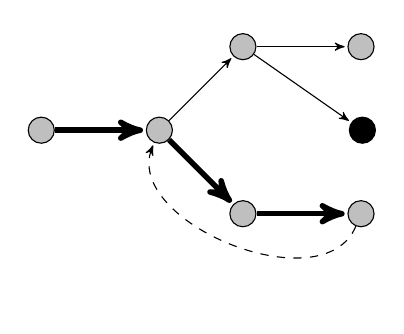
\begin{tikzpicture}[->,>=stealth',shorten >=1pt,auto,node distance=1.5cm]

\node[dot, fill = black!25] (1) [] {};
\node[dot, fill = black!25, right of = 1] (2) [] {};
\node[dot, fill = black!25, below right of = 2] (3) [] {};
\node[dot, fill = black!25, right of = 3] (4) [] {};
\node[dot, fill = black!25, above right of =2] (5) [] {};
\node[dot, fill = black, below right of =5, xshift = 13] (6) [] {};
\node[dot, fill = black!25, right of =5] (7) [] {};

\path
(1) edge [line width = 2] node {} (2)
(2) edge [line width = 2] node {} (3)
(3) edge [line width = 2] node {} (4)
(2) edge [] node {} (5)
(5) edge [] node {} (6)
(5) edge [] node {} (7)
(4) edge [bend left = 90, dashed] node {} (2);
\end{tikzpicture}
\end{minipage}
\begin{minipage}[c]{0.5\textwidth}
The full path does not contain the injected node.

The algorithm backtracks to the last open choice point.
\end{minipage}

\bigskip

\begin{minipage}[c]{0.5\textwidth}
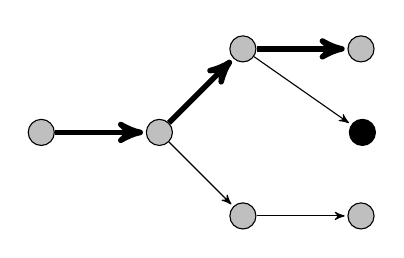
\begin{tikzpicture}[->,>=stealth',shorten >=1pt,auto,node distance=1.5cm]

\node[dot, fill = black!25] (1) [] {};
\node[dot, fill = black!25, right of = 1] (2) [] {};
\node[dot, fill = black!25, below right of = 2] (3) [] {};
\node[dot, fill = black!25, right of = 3] (4) [] {};
\node[dot, fill = black!25, above right of =2] (5) [] {};
\node[dot, fill = black, below right of =5, xshift = 13] (6) [] {};
\node[dot, fill = black!25, right of =5] (7) [] {};

\path
(1) edge [line width = 2] node {} (2)
(2) edge [] node {} (3)
(3) edge [] node {} (4)
(2) edge [line width = 2] node {} (5)
(5) edge [] node {} (6)
(5) edge [line width = 2] node {} (7);
\end{tikzpicture}
\end{minipage}
\begin{minipage}[c]{0.5\textwidth}
DFS resumes its running, until again it reaches a final node.
\end{minipage}

\bigskip

\begin{minipage}[c]{0.5\textwidth}
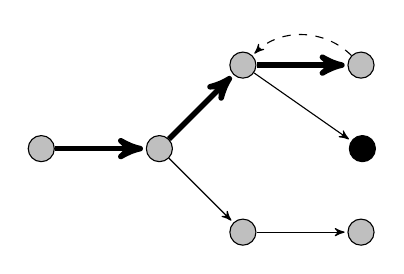
\begin{tikzpicture}[->,>=stealth',shorten >=1pt,auto,node distance=1.5cm]

\node[dot, fill = black!25] (1) [] {};
\node[dot, fill = black!25, right of = 1] (2) [] {};
\node[dot, fill = black!25, below right of = 2] (3) [] {};
\node[dot, fill = black!25, right of = 3] (4) [] {};
\node[dot, fill = black!25, above right of =2] (5) [] {};
\node[dot, fill = black, below right of =5, xshift = 13] (6) [] {};
\node[dot, fill = black!25, right of =5] (7) [] {};

\path
(1) edge [line width = 2] node {} (2)
(2) edge [] node {} (3)
(3) edge [] node {} (4)
(2) edge [line width = 2] node {} (5)
(5) edge [] node {} (6)
(5) edge [line width = 2] node {} (7)
(7) edge [bend right = 45, dashed] node {} (5);
\end{tikzpicture}
\end{minipage}
\begin{minipage}[c]{0.5\textwidth}
Once again, the path is not valid. The algorithm backtracks.
\end{minipage}

\bigskip

\begin{minipage}[c]{0.5\textwidth}
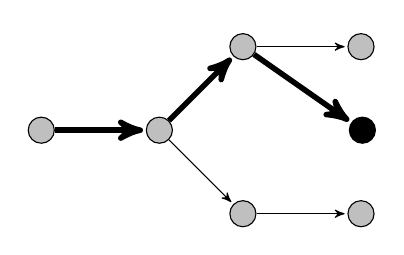
\begin{tikzpicture}[->,>=stealth',shorten >=1pt,auto,node distance=1.5cm]

\node[dot, fill = black!25] (1) [] {};
\node[dot, fill = black!25, right of = 1] (2) [] {};
\node[dot, fill = black!25, below right of = 2] (3) [] {};
\node[dot, fill = black!25, right of = 3] (4) [] {};
\node[dot, fill = black!25, above right of =2] (5) [] {};
\node[dot, fill = black, below right of =5, xshift = 13] (6) [] {};
\node[dot, fill = black!25, right of =5] (7) [] {};

\path
(1) edge [line width = 2] node {} (2)
(2) edge [] node {} (3)
(3) edge [] node {} (4)
(2) edge [line width = 2] node {} (5)
(5) edge [line width = 2] node {} (6)
(5) edge [] node {} (7);

\end{tikzpicture}
\end{minipage}
\begin{minipage}[c]{0.5\textwidth}
The search finds an other complete path. This time the path is acceptable and the process terminates.
\end{minipage}

\bigskip

\bigskip

These two mechanics allow for the definition of two types of contraints: logical constraints that enable/disable nodes, and injections that force the presence of a node in the final output.

The first is used to ensure semantic consistency in the construction of a scene. 

The latter is particularly useful to ensure that the generated story actually contains the set of activities that are to be presented to the final user. This is done by injecting the corresponding nodes so that they become part of the final result. This will be explained in more depth in the next sections.

\bigskip

The behaviour of the graph traversal algorithm can be altered and tuned by changing the policy used to select the next node to be visited. All graph traversal algorithms use a data structure called \textit{Fringe}, or \textit{Frontier}, which holds all the potential "next" nodes to be visited. At each step one of these is selected and the traversal proceeds from it.

Four different selection functions have been implemented and are available:

\begin{itemize}\setlength{\itemsep}{0pt}
\item \textbf{Pure DFS}: the next node to be explored is the furthest away from the starting node. If multiple nodes share the same distance from the origin, one of them is selected at random.
\item \textbf{Pick First}: This policy is mostly for debugging purposes: a predictable version of DFS in which nodes are picked in order.

The ordering on the nodes is defined as a side effect of how the graph structure is stored, and reflects the order in which nodes were added to the graph. 
\item \textbf{Random Search}: the next node is picked at random.
\item \textbf{Inverse Frequency}: this is intended to be the primary selection policy to be used. The Plot Generation Layer keeps memory of how many times each node was used: both in the current story generation process (local frequency) and in all the stories generated by the system in the past (global frequency). Using this policy, a "roulette wheel" selection is used, in which the probability assigned to each node is inversely proportional to their frequency.

The rationale between this system is that, this way, generated plots will be as variable and differentiated as possible, without being predictable.
\end{itemize}
The setting of the desired node selection policy can be done by appropriately from the "configuration.cfg" file.

\bigskip

Summarising, this module uses a pre-defined graph structure to generate a sequence of nodes describing a scene, belonging to a classification of scenes/functions close to that defined by Propp. 

A variant of a DFS search is performed on the graph in a way that ensures adherence to constraints about consistency and content, while trying to minimise repetitivity and predictability.

\pagebreak

\section{Linear Plot Generation}
The module explained in the previous section generates a single scene, from the corresponding probabilistic graph. In order to generate an entire Plot, it is necessary to chain together multiple scenes appropriately.

\bigskip

A \textit{Linear Plot} is the simplest form of plot: a pre-defined sequence of scenes. A specific module takes such a sequence as input, and outputs the corresponding sequence of events.

This operation is carried out iteratively: each scene is processed into a node sequence describing it. At each step, the output is chained with the node sequences produced previously. Then, the next scene is processed, until the list of scenes terminates.

The output is a chain containing the nodes describing each scene, in order.

\subsection{STRIPS State Encoding And Dependencies}
What happens within a scene has repercussions on what happens in others, further down the line. 

For instance, if in the scene mentioned above, corresponding to the \textit{First Function of the Donor} function, the Hero acquires the servitude of the Donor, this allows the hero to be guided to its destination by the Donor in the \textit{Guidance} scene. 

Conversely, if the Hero had failed in acquiring the help of the Donor, the same chain of events describing how the Hero is guided by him could not be followed.

\bigskip

This means that it is necessary to propagate some information from within the generation of a scene to other scenes downstream. This is accomplished through the definition of a State component that receives, stores and provides access to this kind of information.

\bigskip

The State is modelled in a way that loosely follows the STRIPS standard \cite{strips}. STRIPS is a framework for the definition of agents for the resolution of AI problems through planning. It included the definition of a "State of the problem" structure, which was implemented exploiting mechanics typical of logic / functional programming.

Since this work was developed in Java, and since the level of flexibility required was not as high as for a generic planning agent, a simplified version of the STRIPS encoding was used to define the state of the Plot generation.

\bigskip

The state is a collection of objects resembling logic predicates. While logic predicates are flexible in their structure, the predicates in use here are fixed as a \(<String,String>\) pair. The first parameter defines what type of information is being represented, while the second represent its content.

For example, the predicate \(<test\_outcome, success>\) states that the test performed by the Hero in order to gain the help of the Donor had a positive outcome.

\bigskip

Nodes belonging to any function can be associated with pre and postconditions regarding the state: in order for a node to be valid and usable, the preconditions must be respected. If a node is actually used in the scene, its postconditions are applied to the state.

\bigskip

Pre and postconditions take the form of logic expressions on predicates. An ad-hoc group of classes has been implemented to imitate basic mechanics of a logic programming language, including predicate matching, full first-order logic expressions on the matching of predicates, and "universal unification": a value which matches any other value. By using these functionalities, one can easily specify complex dependencies between nodes, even when they belong to different functions.

\bigskip

As a minimal example in the following table is presented the set of conditions necessary to specify two dependencies: the Hero can be guided to his destination by the Donor only if he successfully acquired his servitude by passing a test. At the same time the Hero can fail in finding his way only if he isn't currently being helped by the Donor.

\begin{table}[H]
\caption{Dependency Specification}
\label{tab:dependency}
\bigskip
\begin{tabular}{| l | l | l | l |}
\hline
Label & Interpretation & Cond. Type & Condition \\
\hline
success & the hero passes the test& POST & \(<test\_outcome,success>\) \\
 & devised by the Donor&  & \\
\hline
guidance & the hero is guided & PRE & \(<test\_outcome,success>\) \\
 &by the Donor&  & \\
\hline
guidance\_failure & the hero fails in & PRE & \(NOT<test\_outcome,success>\) \\
 & finding the way&  & \\
\hline

\end{tabular}
\end{table}

As explained in section 5.1.2, during the traversal of a graph defining a function / scene, the preconditions of all nodes are evaluated, ensuring that the final sequence of nodes produced in output contains no invalid nodes. Once a node is added to the path its postconditions are put in effect, affecting the state of the generation.

\pagebreak

\section{Non-linear Plot Generation}
A Linear Plot is clearly too limited and uninteresting: the same sequence of scenes repeats itself unchanged in each generated story.

To address this, a set of mechanics are in place to introduce a higher degree of variability in the story generation process, based on the concept of \textit{Subplots}. 

\bigskip

A Subplot is a new linear plot introduced within an other, to respond to a specific issue. During the generation of a Plot, some story events would prevent the storyline from continuing: for instance, if the Hero fails in finding his way to the Villain, the part of the story in which the two engage in a fight, and eventually the villain is defeated can not take place.

These events are given the name of \textit{Impasses}. They are part of the graphs describing functions, and so they can become part of the story. Once they are, they constitute an obstacle to the linear flow of the storyline.

A subplot must be introduced in which the obstacle is removed. Continuing with the example given above, if the Hero fails in finding his way to the Villain, a subplot is required in which he resumes his travelling and eventually tries again.

\subsection{Impasses}

A specific component, the \textit{ImpasseScanner}, can be set with two different kinds of impasse definitions. The component scans a scene path after it has been produced and before generating the next one.

\begin{itemize}\setlength{\itemsep}{0pt}
\item \textbf{Node labels}: if certain label is found in the path, declare an impasse.
\item \textbf{State properties}: if a certain condition regarding the state is true, declare an impasse.
\end{itemize}

For instance, in order to define the impasse caused by the Hero failing at finding his way to the Villain's location, one could specify the label of the corresponding node, \(guidance\_failure\), or or a logic condition which is true whenever the postconditions of that node are true.

Once an impasse is detected by the ImpasseScanner, the generation process is paused. An other component, the \textit{ImpasseHandler}, receives information describing the impasse and introduces a subplot in order to remove the obstacle.

\bigskip

\subsection{Impasse Handling and Subplots}
The role of the ImpasseHandler is to receive information about an impasse, and launch the generation of a subplot appropriate to resolving it.

This requires a set of subplots to be defined by an author, as well as a mapping between impasses and subplots. Subplots are defined as sequences of scenes / functions, while the mapping is defined directly within the ImpasseHandler component.

\bigskip

Returning to the same example, the \textit{Guidance} function has been generated. The resulting sequence of nodes contains one in which the Hero fails in finding his way to the Villain. The ImpasseScanner detects this and raises an Impasse, passing it to the ImpasseHandler.

Injections can be used to force scenes to develop in a direction that is appropriate to the subplot

The handler accesses the mapping between impasses and subplots, and picks the appropriate subplot object: \textit{RETRY\_GUIDANCE}, defined as follows.

\bigskip

\begin{table}[H]
\caption{The RETRY\_GUIDANCE Subplot}
\label{tab:subplot}
\bigskip
\begin{tabular}{| l | l | l |}
\hline
Function & Possible Developments & Injections \\
\hline
\textit{Filler} & Filler scene. Introduces a new subplot. & \textit{hero\_retry*} \\
\hline
\textit{FirstFunctionReaction} & The Hero meets a Donor character, & \\
 & is tested, and may or may not pass said test. & \\
\hline
\textit{Acquisition} & Consequences of the test: & \\
 & the Donor may or may not help the Hero. & \\
\hline
\textit{Guidance} & The Hero tries to find a way to the Villain. &\\
 & He can be helped by the Donor or by an item&\\
 & given him by the Donor. &\\
\hline
\end{tabular}

\bigskip

* this forces the graph traversal algorithm to output a scene path containing the node \textit{hero\_retry}, in which the Hero decides to make a new attempt at the task he was pursuing earlier.
\end{table}

\bigskip

It is possible that one or more impasses occur in a subplot. The whole mechanic is recursive: a subplot can be interrupted by an impasse, and an other subplot is introduced to clear it.

\begin{figure}[H]
\caption{Recursive Subplots}
 \label{fig:subplots}
 
 \bigskip
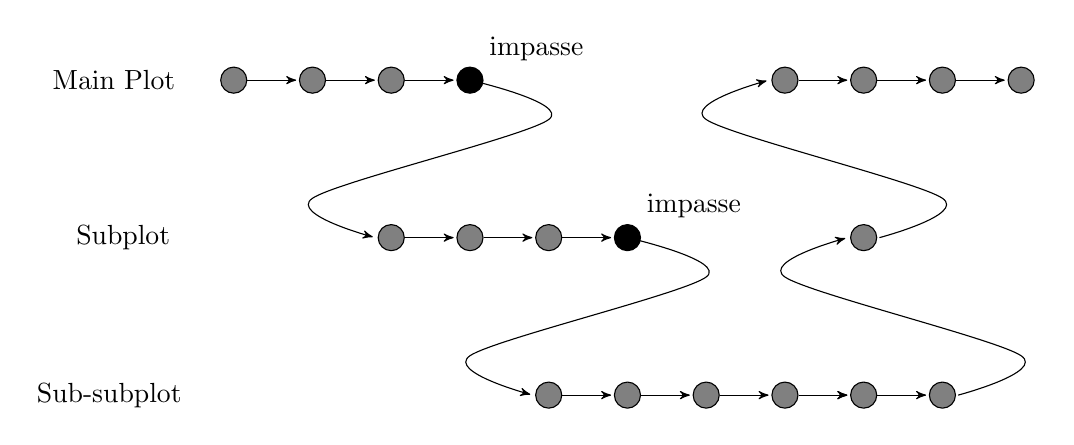
\begin{tikzpicture}[->,>=stealth',shorten >=1pt,auto,node distance=1cm]

%\node [invis, text width = 2cm, name = intro] {donor\\introduction};
\node[dot, fill = black!50] (1) [] {};
\node[dot, fill = black!50, right of = 1] (2) [] {};
\node[dot, fill = black!50, right of = 2] (3) [] {};
\node[dot, fill = black, right of = 3, label={[align=left]above right:{impasse}}] (4) [] {};
\node[dot, fill = black!50, right of = 4, xshift = 3cm] (5) [] {};
\node[dot, fill = black!50, right of = 5] (6) [] {};
\node[dot, fill = black!50, right of = 6] (7) [] {};
\node[dot, fill = black!50, right of = 7] (8) [] {};
\node[invis, left of = 1, xshift=-0.3cm, text width = 2cm, name = l1] {Main Plot};


\node[dot, fill = black!50, below of = 3, yshift=-1cm] (11) [] {};
\node[dot, fill = black!50, right of = 11] (12) [] {};
\node[dot, fill = black!50, right of = 12] (13) [] {};
\node[dot, fill = black, right of = 13, label={[align=left]above right:{impasse}}] (14) [] {};
\node[dot, fill = black!50, right of = 14, xshift = 2cm] (15) [] {};
\node[invis, below of= l1, xshift=0.3cm, yshift=-1cm, text width = 2cm, name = l2] {Subplot};

\node[dot, fill = black!50, below of = 13, yshift = -1cm] (21) [] {};
\node[dot, fill = black!50, right of = 21] (22) [] {};
\node[dot, fill = black!50, right of = 22] (23) [] {};
\node[dot, fill = black!50, right of = 23] (24) [] {};
\node[dot, fill = black!50, right of = 24] (25) [] {};
\node[dot, fill = black!50, right of = 25] (26) [] {};
\node[invis, below of= l2, yshift=-1cm, text width = 3cm, name = intro] {Sub-subplot};

\path
(1) edge [] node {} (2)
(2) edge [] node {} (3)
(3) edge [] node {} (4)
(5) edge [] node {} (6)
(6) edge [] node {} (7)
(7) edge [] node {} (8);

\path
(11) edge [] node {} (12)
(12) edge [] node {} (13)
(13) edge [] node {} (14);

\path
(21) edge [] node {} (22)
(22) edge [] node {} (23)
(23) edge [] node {} (24)
(24) edge [] node {} (25)
(24) edge [] node {} (25)
(25) edge [] node {} (26);

\draw plot [smooth] coordinates {(3,0) (4,-0.5) (1,-1.5) (1.8,-2)};
\draw plot [smooth, yshift=-2cm, xshift=2cm] coordinates {(3,0) (4,-0.5) (1,-1.5) (1.8,-2)};
\draw plot [smooth] coordinates {(9.2,-4) (10,-3.5) (7,-2.5) (7.8,-2)};
\draw plot [smooth, yshift=2cm, xshift=-1cm] coordinates {(9.2,-4) (10,-3.5) (7,-2.5) (7.8,-2)};

\end{tikzpicture}
\end{figure}

\bigskip

One problem that is immediately apparent is that there is no guarantee that the recursion will terminate. In theory it would be possible that each successive subplot keeps running into an impasse and introducing an other and so on, in an infinitely deep nesting.

\bigskip

In practice this is resolved by the node selection policy used in the graph traversal procedure. As explained in 4.1.2, the default policy selects the next available node according to a probability distribution in which nodes that have already been used in the story are less likely to be picked. The probability decreases each time the node is used.

Impasses depend on the usage of specific nodes, and since every time an other level of recursion is called one of these nodes is used, the probability of impasses occurring decreases with the depth of the recursion and with the length of the story. 

As a consequence, impasse-causing nodes are unlikely to be picked deep in the recursion nesting, as well as down along the story. This means that every impasse will eventually be cleared and the generation algorithm will be allowed to terminate.

\bigskip

Once the generation of main plot terminates, the entire Plot Generation process terminates, producing in output a sequence of nodes as the concatenation of all the function/scene paths generated, in order.

\pagebreak

\chapter{Text Generation}
The previous chapter explains how the Plot Generation Layer of the system generates a sequence of nodes, each of which describing a story event, linked to one another.

This sequence is the input to the Text Generation Layer, which will then process it into readable text.

\bigskip

The main obstacle to be overcome during this step derives from the lack of semantics in the input. This is because the nodes that compose it lack any semantic meaning. This in turn derives from the process from which they originated.

These nodes come from the graph structures described in the previous chapter. A human author has designed these graphs. Each one of them models the different ways in which a scene can unfold. This in turn means that these graphs have been designed with a semantic meaning. 

However, this semantic information is not carried within the nodes, but rather in its interpretation in the mind of the human author. This interpretation is not encoded in the structure of nodes and is therefore lost as soon as the graph is defined.

The main role of this Text Generation Layer is to add again semantic value to these events, resulting in a readable, and meaningful, output.

\bigskip

The option of encoding the semantic meaning of each node within its structure was considered and discarded. It was discarded because of two reasons:

\begin{itemize}\setlength{\itemsep}{0pt}
\item It would make the association between node and semantic static. A dynamic definition makes it possible to change of the semantic information associated to nodes on demand. even at runtime.
\item The definition of graph structure and the nodes they contain is already rather delicate. Requiring the definition of semantics within it would make it even more complex.
\end{itemize}

As a consequence, the definition of the semantic meaning of a node takes place after the plot sequence has been generated by the first layer.

This is achieved through the definition of \textit{Text Dictionaries}, that associate nodes with short pieces of symbolic text. These texts are not in the final form of the output, and need to be processed further, but manage to provide semantic information to nodes. For each node, the dictionary associates its label to an array of pieces of text.

Definition and properties of these text dictionaries, and how they are used by the Text Generation module are explained in the next section.

Moreover, this layer provides linking to the Story Space (see chapter 2), by introducing existents appropriately. Ths mechanic will be the subject of section 6.1.2.

\pagebreak

\section{From Nodes to Text}
The algorithm that processes the node sequence into readable text proceeds as follows:

\begin{enumerate}\setlength{\itemsep}{0pt}
\item As a first step, the sequence is parsed and each node is processed into a \textit{TextElement}. Different subclasses of TextElement carry out specific different roles in the writing of the final text.
\item The sequence is filtered, removing all those TextElements coming from nodes that were a by-product of the generation process, but that are not to be transformed into text. 

These nodes were introduced during plot generation to prevent some errors from occurring, for debugging purposes and to allow useful logging of the procedure. Since they are no longer needed, these TextElements are screened out and discarded. 

Any other node, whose role is yet to be determined, is of the \textit{StringElement} type.
\item For each String Element, a first expansion step is performed:
\begin{enumerate}\setlength{\itemsep}{0pt}
\item The node label is used to retrieve one of the pieces of text defined in the text dictionary mentioned above, at random. This adds the semantic meaning carried by a dictionary entry into the system again.
\item Each word in this text is processed back into subclasses of TextElement: words that are all in upper case are made into ExistentElements, which will later be processed into ground existent instances. All other words are made into PlainElements, simple wrappers for a string.
\item The resulting subsequence of TextElements substitutes the single TextElement from which it originated, in the main sequence.
\end{enumerate}
\item The expanded sequence is parsed again, this time processing each TextElement into an actual word. PlainElements are resolved to their original string value, while ExistentElements are resolved to the name of an existent.

The process through which ExistentElements are given their definitive form is subject of the next section.
\end{enumerate}

\begin{figure}[H]
\caption{The Text Generation Process}
 \label{fig:fabulamodel}
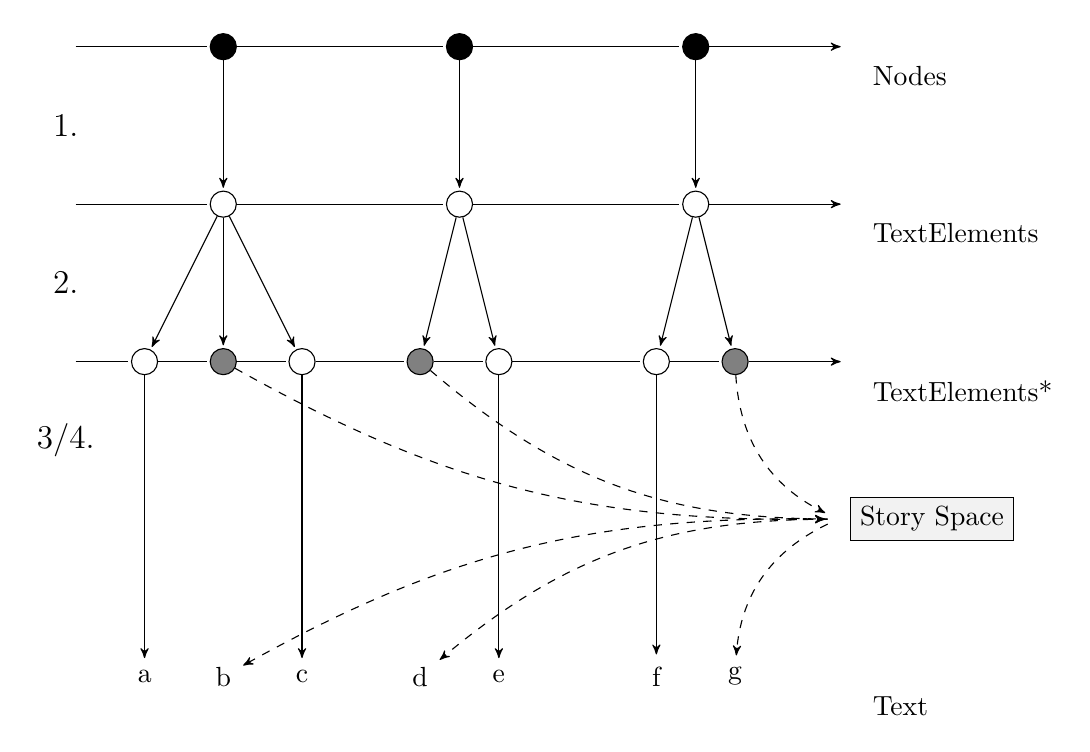
\begin{tikzpicture}[->,>=stealth',shorten >=1pt,auto,node distance=1cm]

\node[invis, xshift = -2cm] (a0) [] {};
\node[dot, fill = black] (a1) [] {};
\node[dot, fill = black, xshift = 3cm] (a2) [] {};
\node[dot, fill = black, xshift = 6cm] (a3) [] {};
\node[invis, xshift = 8cm, label={[align=left] below right:{Nodes}}] (a4) [] {};
    
\path
(a0) edge [-] node {} (a1)
(a1) edge [-] node {} (a2)
(a2) edge [-] node {} (a3)
(a3) edge [] node {} (a4);

\node[invis, yshift=-2cm, xshift=-2cm] (b0) [] {};
\node[dot, fill=white, yshift=-2cm] (b1) [] {};
\node[dot, fill=white, yshift=-2cm, xshift=3cm] (b2) [] {};
\node[dot, fill=white, yshift=-2cm, xshift=6cm] (b3) [] {};
\node[invis, yshift=-2cm, xshift = 8cm, label={[align=left] below right:{TextElements}}] (b4) [] {};

\path
(b0) edge [-] node {} (b1)
(b3) edge [] node {} (b4)
(b1) edge [-] node {} (b2)
(b2) edge [-] node {} (b3);

\path
(a1) edge [] node {} (b1)
(a2) edge [] node {} (b2)
(a3) edge [] node {} (b3);

\node[invis, yshift=-4cm, xshift=-2cm] (c0) [] {};
\node[dot, fill=white, right of = c0] (c1) [] {};
\node[dot, fill=black!50, right of = c1] (c2) [] {};
\node[dot, fill=white, right of = c2] (c3) [] {};
\node[dot, fill=black!50, xshift=0.5cm, right of = c3] (c4) [] {};
\node[dot, fill=white, right of = c4] (c5) [] {};
\node[dot, fill=white, xshift=1cm, right of = c5] (c6) [] {};
\node[dot, fill=black!50, right of = c6] (c7) [] {};
\node[invis, right of = c7, xshift=0.5cm, label={[align=left] below right:{TextElements*}}] (c8) [] {};

\path
(c0) edge [-] node {} (c1)
(c1) edge [-] node {} (c2)
(c2) edge [-] node {} (c3)
(c3) edge [-] node {} (c4)
(c4) edge [-] node {} (c5)
(c5) edge [-] node {} (c6)
(c6) edge [-] node {} (c7)
(c7) edge [] node {} (c8);  

\path
(b1) edge [] node {} (c1)
(b1) edge [] node {} (c2)
(b1) edge [] node {} (c3)
(b2) edge [] node {} (c4)
(b2) edge [] node {} (c5)
(b3) edge [] node {} (c6)
(b3) edge [] node {} (c7);

\node[block, right of = c7, xshift=1.5cm, yshift=-2cm] (Dict) [] {Story Space};
\node[invis, right of = c7, xshift=0.3cm, yshift=-2cm] (D) [] {};

\node[invis, yshift=-8cm, xshift=-2cm] (d0) [] {};
\node[invis, right of = d0] (d1) [] {a};
\node[invis, right of = d1] (d2) [] {b};
\node[invis, right of = d2] (d3) [] {c};
\node[invis, xshift=0.5cm, right of = d3] (d4) [] {d};
\node[invis, right of = d4] (d5) [] {e};
\node[invis, xshift=1cm, right of = d5] (d6) [] {f};
\node[invis, right of = d6] (d7) [] {g};
\node[invis, right of = d7, xshift=0.5cm, label={[align=left] below right:{Text}}] (d8) [] {};

\path
    (c1) edge [] node {} (d1)
    (c3) edge [] node {} (d3)
    (c5) edge [] node {} (d5)
    (c6) edge [] node {} (d6)
    (c2) edge [dashed, bend right = 15] node {} (D)
    (D) edge [dashed, bend right = 15] node {} (d2)
    (c4) edge [dashed, bend right = 20] node {} (D)
    (D) edge [dashed, bend right = 20] node {} (d4)
    (c7) edge [dashed, bend right = 30] node {} (D)
    (D) edge [dashed, bend right = 30] node {} (d7);
    
\node[invis, below of = a0] (one) {\large{1.}};
\node[invis, below of = b0] (two) {\large{2.}};
\node[invis, below of = c0] (three) {\large{3/4.}};

\end{tikzpicture}
(*)some of which are ExistantElements, in grey;
\end{figure}

As an example, here is given an example of the series of steps that transform a node label into a short piece of text.

\begin{table}[H]
\caption{Processing a Node into Text}
\label{tab:expansion}
\bigskip
\begin{tabular}{| l | l |}
\hline
Data Type & Value \\
\hline
\textit{Label} & "fight" \\
\hline
\textit{StringElement(SE)} & SE(fight) \\
\hline
\textit{string} & "HERO and VILLAIN engage in combat" \\
\hline
\textit{ExistentElement(EE)/} & EE(HERO),PE(and),EE(VILLAIN),PE(engage),\\
\textit{PlainElement(PE)} & PE(in),PE(combat) \\
\hline
\textit{string} & "The knight and the evil witch engage in combat." \\
\hline

\end{tabular}
\end{table}

The final story text is the concatenation of all the texts resulting from the node sequence.

\subsection{Space and Existents}
The pieces of text associated to plot nodes contain a certain degree of indetermination. Existents are not defined, and are only referenced to as variables.

The text given above, \textit{"HERO and VILLAIN engage in combat"}, is an example of this: \textit{HERO}, and \textit{VILLAIN} are keywords that identify a class of existent. In the final text, these keywords will be substituted by ground instances of this class.

\bigskip

The instantiation of existents belong to the Space of the story. Two are the steps that need implementation: first it is necessary to define what specific existent will be the ground instance of the class and second, consistency must be ensured, even considering the fact that there can be multiple instances of the same class. 

There can be multiple Donor characters, for instance, interacting with the hero in different moments fo the story.

A system is implemented to provide these two steps in a modular and customisable way.

\bigskip

First of all, a simple classification of existents was given, based on the classification given by Propp.

\begin{itemize}\setlength{\itemsep}{0pt}
\item \textit{Hero, Villain, Donor, Dispatcher, False Hero}: these are borrowed directly from Propp's ontology, as explained in chapter 1.
\item \textit{Victim}: this class was introduced to group together all those characters that can be victim to the Villain's misdeed.
\item \textit{Location, Item}. Propp's classification only considered characters. Places and physical objects are also existents and have to be part of the Space.
\end{itemize}

Then, a dictionary file is populated with a set of possible instances for each class. Just to give a few examples, instances of the class \textit{HERO} can be something like \textit{The Knight, the Prince, Boris, Ivàn}, and so on. 

\bigskip

The definition of these instances in a separate file allows for a quick change of setting. If, instead of generating stories with a classic folktale setting, one was to generate narrative set in science-fiction space setting, this would simply require to swap out one dictionary for an other, defining the new setting.

\bigskip

The first step of the process, in which the ground instance of the existent class is determined, becomes really simple: an instance is selected at random from the dictionary.

\bigskip

Then it is necessary to ensure consistency. Once it is determined that the Hero will be \textit{Boris}, this must hold until the end of the story, rather than randomising it again every time the variable \textit{HERO} is encountered.

Some variables should only be randomised once. There is only one hero, and only one villain, for instance.

Others can, and should, be randomised multiple times. Multiple items will appear during the course of the narration, multiple locations and multiple donors.

\bigskip

This is achieved by keeping track of the state of the Text generation process, by the means of the same system used during Plot generation (section 5.2.1).

Predicates are used to encode information about the instantiation of existents. This information is generated when the randomisation takes place, and propagates forward during the parsing process.

When an existent is randomised, a predicate in the form \(<Class,Instance>\), such as \(<HERO,Boris>\) is added to the State. From this point downstream, every time an existent variable is encountered for the class \textit{HERO}, its value is known and it can be substituted without randomisation.

\bigskip

Still, this is not sufficient, because some existents do need to be randomised again multiple times.

\bigskip

A solution to this issue comes from the recursive structure of the plot generation algorithm: the existents that need to be randomised again are those introduced in subplots. For instance, if the hero fails in passing a test devised by a donor, a subplot will be introduced in which he will meet a new one.

In order to follow the recursive structure of the plot, a stack of state objects is used instead of a single one. Whenever the parsing encounters the beginning of a subplot, a new state is added to the stack, containing the predicates of the parent state, filtered to remove those describing existents that need to be randomised again in this subplot.

When the subplot terminates, the sub-state is merged back into that of the parent plot and removed from the stack.

\bigskip

This mechanic may seem an overcomplicated way to meet the requirements: a simpler way to achieve the same result would have been to introduce a numbering in the existents, and distinguish an instance from the other already at generation time.

For instance, the first item to be part of the story would have been \textit{ITEM1}, then in the next subplot \textit{ITEM2} and so on. This way, consistency between occurrence of the same instance would be maintained, while different instances would have been easily detected and re-randomised.

\bigskip

However, the system currently in place is much easier to expand, in the context of any future development of this work. 

The hooks it provides in correspondence to the introduction and resolution of a new subplot allow for a stricter and deeper interaction with the state of the generation process, to be used in any more advanced text generation algorithm.

\pagebreak

\section{Final Output}
The final output is a .json file. It contains an array of Json Objects, each of which has four fields:

\begin{itemize}\setlength{\itemsep}{0pt}
\item \textit{label}: the label of a story node, from the plot sequence. 
\item \textit{text}: the line of text produced from said node, in its ground, resolved, form.
\item \textit{node\_type}: the class under which the node falls, following the simplified classification explained in 4.1.
\item \textit{activity}: the identifier of an activity, or \textit{null} if no activity is associated to this node. Only the activities specified in input will appear in the output.
\end{itemize}

The length of the array varies, according to the variability inherent to the plot generation algorithm. With the current, "proof of concept", settings it varies between 75 and 150 elements.

\pagebreak

\chapter{Conclusions}
In conclusion, this work presents a new approach for Constrained Story Generation (see 2.1: \textit{The Mixed Initiative approach}), based on a two-layered architecture.

The Plot Generation layer works on two levels of abstraction, in parallel: human-authored probabilistic graphs model scenes (4.1), while a recursive algorithm determines the sequence of scenes to be generated, introducing new subplots to resolve impasses in the generation process (4.2 to 4.3).

An encoding of the State of the generation, based on principles borrowed from classic AI (see 5.2.1: \textit{STRIPS State Encoding}) and logic programming, is used to ensure the adherence to constraints and specifications regarding the output.

\bigskip

The output of this layer is used by a Text Generation layer, which re-introduces semantic meaning using a human authored dictionary (5.1) and a stack-like structure to model the State of the text generation, in order to properly substitute keywords with the name of existents (5.1.1).

\bigskip

This approach has a few characteristics that make it different from others already present in literature:

\begin{itemize}\setlength{\itemsep}{0pt}
\item It is one of the very few attempts at generating Constrained Plot and Constrained Space (see 2.2). Among the other examples of this level of automation, it is the only one not to be based on character simulation, and the only one that doesn't require a human to be present during the generation process.
\item It is the only approach based on the cooperation between two different levels of abstraction: one at a high level, based on Prop's research, and one at a lower level, based on the Fabula Network Model.
\item The high degree of modularity allows for customisation, flexibility and expansion of the system.
\end{itemize}

At the same time, the system shows a clear limitation, being the amount of authorial work that is required prior to the actual generation process.

In particular, in order to launch an effective generation process, a human author needs to define the following:
\begin{itemize}\setlength{\itemsep}{0pt}
\item A set of scenes composing the main plot, and a number of scene sequences describing subplots. Currently the set of Functions defined by Propp is being used, but the system can work with any group of scenes.
\item A probabilistic graph structure for each scene, defining the different events that can happen. Again, in the current implementation these are based on the definition of scenes given by Propp.
\item Proper logic rules to ensure consistency within a scene and between scenes.
\item Impasses, and the subplots to be introduced to solve them.
\item A Text Dictionary, carrying the semantic information to be associated to node labels.
\end{itemize}

Especially the design and input of graph structures are particularly demanding tasks. The specific way in which the data are coded will be explained in appendix B.

This step requires the author to decide in what ways a scene can develop, code this information into a graph with the appropriate language, and define the appropriate rules to ensure consistency in the results.

Given that the system cannot generate anything outside the space given to it as knowledge base, the quality and variety of generated stories depends on the quality and volume of the inputs. For this reason, quality in the output requires a substantial investment in the authorial phase.

\bigskip

The ways in which these limits can be improved upon or overcome are part of the next section.

\pagebreak

\section{Further Developments And Improvements}

The result of this work is not a complete product. Some developments are needed in order to make it usable in the context of projects like MoveCare or REWIRE (see chapter 1). Moreover, it could benefit from a few improvements that would make it more effective in fulfilling its role.

\bigskip

\subsection{Necessary Refinements}

In order to make this architecture usable in a real-world application, it is first of all necessary to further develop the Text Generation step. The current system (see Appendix A for examples) is sufficient to show that semantic information can be re-introduced in the story structure, but is too primitive to generate text that can be considered interesting by a user.

The generation of complex text, or the \textit{Discourse} (see chapter 2) of a story, is a vast subject, with many open questions, difficult to undertake. 

The proposed way to develop the system in order to overcome this obstacle is to convey the output to the user partly in the form of text, and partly in the form of animated images.

It is certainly possible to compose simple, 2-dimensional, animations based on the short texts used to define the semantic meaning of node labels. 

\bigskip

For instance, starting from a database of sprites and animations, a piece of text like \textit{the knight and the witch engage in a fight} can be used to generate and show a short animated clip of a knight and a witch fighting. The same can apply to many more events of the story.

At the same time, some text is still required. In some cases the events narrated don't translate well into an animation: \textit{the prince reflected upon the problem} would probably translate into an uninteresting animation, for instance. 

Also, having images or animations accompanied by text would be the preferred way of presenting a story and, while requiring less text than a text-only presentation, would still require a refinement of the text generation procedure.

\bigskip

A first, relatively inexpensive step would be the expansion and partial rewriting of the text dictionary. Adding more descriptive, and perhaps more interesting, pieces of text. This task is beside the scientific goals of this work, and therefore has not being tried at the moment of writing.

\bigskip

Whether it be for the purpose of a more advanced text generation, or as a step in generating images / animations, the preliminary step should be the definition of an ontology representing (and coding) the different classes of existents, their properties, and the relationship between them.

This structure should be usable at runtime to associate together characters, locations, items and animations in way that ensures a more interesting characterisation of any existent. 

For instance, a certain character could be associated to a set of items that he owns and that can be displayed in an image or in the text introducing it. It could be associated to a location where he lives and where he interacts with the hero. Different existents could have properties defined for them that describe how they interact with other existent, how they can be used in the story, how they can be animated, and so on.

\bigskip

An other student is currently working on this specific task. Since he started very recently it was not possible to include any account of his work in this thesis.

\bigskip

\subsection{Suggestions on Further Research}
In order to test the effectiveness of this system in promoting the engagement of users in a set of activities with the goal of improving their health, it is required to develop a complete prototype and to deploy it in the context of a project such as the ones described in chapter 1. Following the timings and schedules of a clinical trial.

However, this is not necessary for the testing of the system as a pure story generation architecture.

Here is proposed a process to determine whether the system is successful in generating acceptable stories, through crowdsourcing.

\begin{enumerate}\setlength{\itemsep}{0pt}
\item The generator is used to produce a set of stories.
\item A set of real-world tales is selected. 
\item These stories are decomposed by hand into sequences of the same texts defined in the text dictionary. This way they will be indistinguishable from generated stories in terms of language. Whatever differences in structure and existents remain.
\item A set of stories of the same size is generated.
\item A set of existents is composed, containing some from the real-world stories and others that did not appear in them. Ensuring that enough foreign existents are part of the set will make real stories less recognisable.
\item Existents in the two groups of stories are scrambled.
\item A sample containing both groups, shuffled, is presented to a crowd", of sufficient size. Subjects are asked to estimate how much each story seems "real" or "fake", and why.
\end{enumerate}

This process should highlight any differences in the structure of stories, between real and generated ones. Differences in language and existents should have been removed by the translation and scrambling steps.

If this quality evaluation proves to be effective in highlighting these differences, it could be employed to refine the system iteratively, thought multiple iteration of testing and a refinement steps.

\bigskip

The procedure is just outlined here: some steps are not entirely defined. In particular the process of decomposition of a real tale into the language used by the generator requires once again authorial work by a human, who would need to face part of the obstacles emerged during the failed attempt at story generation explained in chapter 3.

This step is however necessary. Without the development of a \textit{perfect}, Discourse generation system, indistinguishable from a human, generated stories and real one would always be recognisable by the differences in their Discourse: the language used, the ordering of the events, the way in which they are recounted, the rhythm of the narration and such.

\bigskip

An other potential area of exploration that is opened by the outlining of this architecture is the automation of the authorial task of defining the graph structure describing scenes.

Fruitful work in this direction would greatly improve the effectiveness of this approach, by significantly reducing the amount of authorial work required for the initialisation of the system. In turn this would make the system a great deal more flexible, because it could automatically adapt to a new dataset of stories, or a more sizeable one.

The first obstacle to any research on the subject would be the lack of datasets with annotations of sufficient size. Possibly crowdsourcing can offer an answer in this sense as well.

\appendix

\chapter{Examples}
Below are shown two examples of generated stories. This is not a representation of the full output but rather only of the output text data. Node label, node type and proposed activities are not reported.

Titles have been generated by adding a special node containing the text \textit{HERO and VILLAIN}. This node is then processed like any other, so the variables are resolved to ground existents.

This procedure is by no means final, but it is still useful to give some context, albeit crude, to the story, by introducing the main characters.

\section{Prince Boris and the Black Knight}

\begin{longtable}[H]{| p{0.5\textwidth} | p{0.5\textwidth} |}
	\caption {Prince Boris and the Black Knight}\\
\hline
prince Boris lives at the tower & the hero is introduced\\
\hline
the Black Knight demands the old man to be murdered & \\
\hline
the demand is accepted & \\
\hline
the old man is murdered & \\
\hline
the Black Knight goes in hiding at the tower & \\
\hline
vengeance is required & \\
\hline
the king sends prince Boris on the mission & \\
\hline
prince Boris prepares & \\
\hline
the quest begins&  \\
\hline
prince Boris departs & \\
\hline
prince Boris reaches the tower & \\
\hline
at the tower lives the hermit & \\
\hline
the hermit attacks prince Boris & \\
\hline
the hermit and prince Boris fight each other & \\
\hline
prince Boris begins the test & \\
\hline
prince Boris has passed the test & no impasse\\
\hline
prince Boris will now be helped by the hermit & \\
\hline
prince Boris finds the magical sword & \\
\hline
prince Boris desires the magical sword & \\
\hline
prince Boris acquires the magical sword & \\
\hline
prince Boris discovers a way to the tower & no impasse\\
\hline
prince Boris follows the path to the tower & \\
\hline
prince Boris arrives to the tower & \\
\hline
prince Boris fights the Black Knight & \\
\hline
prince Boris is victorious & no impasse again\\
\hline
prince Boris is scarred & this event allows the hero to be recognised by the scar\\
\hline
the Black Knight is defeated & \\
\hline
the Black Knight is imprisoned & \\
\hline
prince Boris returns & \\
\hline
prince Boris is returning & \\
\hline
the servant overhears prince Boris talking about his success & \\
\hline
the servant learns of what prince Boris has done & \\
\hline
the servant presents his claims to the king & \\
\hline
the king acknowledges the claims presented by the servant & \\
\hline
the servant is rewarded & impasse: a subplot is introduced\\
\hline
prince Boris presents his claims to the king & \\
\hline
the king listens to prince Boris presenting his claims & \\
\hline
the claims are not accepted & \\
\hline
prince Boris confronts the servant & \\
\hline
prince Boris is recognised by the mark he is carrying & this can only happen if the hero has been scarred\\
\hline
prince Boris is finally recognised & \\
\hline
the servant is exposed & \\
\hline
the reward to the servant is withdrawn & \\
\hline
the servant is punished & \\
\hline
the servant is killed & \\
\hline
prince Boris is rewarded with a magical crown 	& \\
\hline
\end{longtable}

In this first example the hero only runs into one impasse. Every other obstacle is overcome immediately: a sudden aggression is repelled defeated and the aggressor becomes a helper, a magical item is found, the villain is defeated in the first attempt.

When Prince Boris is returning home, however, a servant gains knowledge of what happened and claims the reward in his stead. A subplot is introduced in which the hero is recognised by a bodily mark: a scar inflicted to him during his fight with the villain.

The story then draws to an end: the false hero is exposed and killed, and the Prince is rewarded with a magical item.

The hero being scarred and then recognised is an example of how consistency rules can be used to enable certain events. The postcondition of the node associated to the scarring is the precondition to the one in which the hero is recognised from a bodily mark. This way this can of recognition can only take place if the hero has been previously marked during combat.


\section{The Youth and The Evil King}

\begin{longtable}[H]{| p{0.5\textwidth} | p{0.5\textwidth} |}
\caption {The Youth and The Evil King}\\
\hline
the Evil King hears the Youth from afar & \\ 
\hline
the Youth unwillingly reveals information, upon which the Evil King hatches a plan & \\
\hline
the Evil King seizes the magical bow & \\ 
\hline 
the Evil King runs away to the forest & \\ 
\hline 
the magical bow is needed  & \\ 
\hline
the king announces the misfortune to the Youth  & \\ 
\hline
the Youth acknowledges the problem  & \\ 
\hline
the quest begins  & \\ 
\hline
the Youth departs  & \\ 
\hline
the Youth reaches the forest  & \\ 
\hline
the Pixie is at the forest  & \\ 
\hline
the Youth sees the Pixie  & \\ 
\hline
the Youth wants to catch the Pixie  & \\ 
\hline
the Youth catches the Pixie  & \\ 
\hline
the Pixie begs the Youth  & \\ 
\hline
the Youth begins the test  & \\ 
\hline
the Youth has passed the test  & \\ 
\hline
the Youth will now be helped by the Pixie  & \\ 
\hline
the Pixie gives the magical sword to the Youth  & \\ 
\hline
the Youth acquires the magical sword & \\ 
\hline
the Youth finds a path to the forest  & \\ 
\hline
the Youth follows the path to the forest  & \\ 
\hline
the Youth arrives to the forest  & \\ 
\hline
the Evil King and the Youth fight  & \\ 
\hline
the Youth is unable to effectively fight the Evil King  & \\ 
\hline
the Evil King is victorious  & impasse: the hero has been defeated\\ 
\hline
the Youth barely escapes with his life  & filler: new subplot introduced\\ 
\hline
the Youth resumes his travelling  & \\ 
\hline
the Youth is now at the castle  & \\ 
\hline
the hermit is at the castle  & \\ 
\hline
the Youth is tested by the hermit  & \\ 
\hline
the Youth begins the test  & \\ 
\hline
the Youth has failed the test  & impasse: test failed\\ 
\hline
the Youth understands he has failed the test  & \\ 
\hline
the Youth resumes his travelling  & a subplot is introduced so that the hero can try again\\ 
\hline
the Youth arrives at the tower  & \\ 
\hline
the warrior is at the tower  & \\ 
\hline
the warrior is held in captivity. He sees the Youth approaching  & \\ 
\hline
the warrior wants to be free  & \\ 
\hline
the warrior asks the Youth for freedom  & \\ 
\hline
the Youth begins the test  & \\ 
\hline
the Youth has failed the test  & an other failure. An additional subplot is introduced recursively, in which he will try again\\ 
\hline
the Youth resumes his travelling  & \\ 
\hline
the Youth is now at the mountain  & \\ 
\hline
at the mountain lives the lady of the forest  & \\ 
\hline
the lady of the forest is displaying the flying shoes  & \\ 
\hline
the lady of the forest sees the Youth  & \\ 
\hline
the lady of the forest offers a trade  & \\ 
\hline
the Youth begins the test  & \\ 
\hline
the Youth has passed the test  & success, the impasse is broken\\ 
\hline
the lady of the forest decides to help the Youth  & \\ 
\hline
the Youth is magically transported to the mountain by the lady of the forest & the donor actively helps in enabling the hero's transportation\\ 
\hline
the Youth is finally at the mountain  & \\ 
\hline
the Youth and the Evil King engage in a fight & \\ 
\hline
the magical sword helps the Youth in the fight & the hero can use an item he previously acquired\\ 
\hline
the Youth defeats the Evil King  & \\ 
\hline
the Youth obtains the magical bow & \\ 
\hline
the Youth seizes the magical bow  & \\ 
\hline
the Youth returns  & \\ 
\hline
the Youth has arrived back & \\ 
\hline
the Youth marries & \\ 
\hline
\end{longtable}

In this story, multiple impasses are caused by the hero failing at obtaining the help of various donors. Initially he manages to have a magical sword given to him, by freeing a pixie.

Later he is defeated by the villain and barely escapes. he would try again, but he fails twice in obtaining the help of other characters: he fails in answering to the questions of a hermit, and in freeing a warrior held prisoner in a tow. He then he accepts a trade with the lady of the forest and is transported again by her to the mountain where the villain is hiding. 

\bigskip

In the current implementation the text resulting from these texts is rather dull and repetitive, because the path describing them is meant as a placeholder to indicate that a test is taking place. With more authorial work more detail about these tests could be made part of the graph structure and appear in the story.

\bigskip

The hero then defeats the villain and returns back to get married. In this story no false hero appears, since the hero returns back without divulging information about his deed.



\printbibliography

\end{document}

